%========================================
% PREAMBOLO
%========================================

% === Impostazione del documento ==========================
\documentclass[12pt,a4paper,oneside,onecolunm,english,hidelinks]{book}
\pagenumbering{arabic}
\usepackage{setspace}
\onehalfspace

% === Regolazione dei margini =============================
\addtolength{\oddsidemargin}{30pt}
\addtolength{\evensidemargin}{-30pt}
\usepackage{fancyhdr}
\usepackage{multirow}
\usepackage{multicol}
\usepackage[section]{placeins}

% === Impostazione dei font ===============================
\usepackage[T1]{fontenc}
\usepackage[utf8]{inputenc}
%\usepackage[italian]{babel}
\usepackage[english]{babel}
\usepackage{ae}
\usepackage{relsize}
\usepackage{csquotes} 
\usepackage{amsmath}
\usepackage{amsfonts}
\usepackage{mathdots}
\usepackage{mathtools}
\usepackage[colorlinks=true]{hyperref}
\hypersetup{
	bookmarksnumbered=true,
	linkcolor=black,
	citecolor=black,
	pagecolor=black,
	urlcolor=black,
	pdftex,
    pdfauthor={Argentieri Francesco}
}
\usepackage{verbatim}
\usepackage{alltt,footnote}
\DeclareMathOperator{\sgn}{sgn}
\DeclarePairedDelimiter{\abs}{\lvert}{\rvert}
\DeclarePairedDelimiter{\norma}{\lVert}{\rVert}

% === Integrazione delle figure ===========================
\usepackage{graphicx}
\graphicspath{{./imgs/}}
\renewcommand{\figurename}{Fig.}
%\usepackage{subfigure}
\usepackage{subfig}
\usepackage[dvipsnames]{xcolor}

% === Per gli algoritmi ===================================
\usepackage{algorithmicx}
\usepackage[ruled]{algorithm}
\usepackage{algpseudocode}

% === Per le tabelle ======================================
\usepackage{tabularx}
%\usepackage[table]{xcolor}

%==Per le figure latex======================================
%Package e librerie per TikZ e PGF, le librerie non sono tutte necessarie a questo documento LATEX.
\usepackage{tikz,fp,ifthen,fullpage}
\usepackage{pgfmath}
\usetikzlibrary{decorations.pathmorphing,backgrounds,fit,calc,through}
\usetikzlibrary{arrows}
\usetikzlibrary{shapes,decorations,shadows}
\usetikzlibrary{fadings}
\usetikzlibrary{patterns}
\usetikzlibrary{mindmap}
\usetikzlibrary{decorations.text}
\usetikzlibrary{decorations.shapes}
\usepackage{pgfplots}
\usepgfplotslibrary{colorbrewer}
\usepgfplotslibrary{patchplots}
\pgfplotsset{compat=1.13}

%==Per APDL e linguaggi======================================          
\usepackage{listings,color}
\definecolor{codeBlue}{RGB}{0,0,255}
\definecolor{codeGreen}{RGB}{0,128,0}
\definecolor{codePurple}{RGB}{128,0,255}
\definecolor{codeOrange}{RGB}{255,128,128}
\definecolor{codePink}{RGB}{255,0,255}
\definecolor{codeGray}{rgb}{0.5,0.5,0.5}
\lstdefinestyle{apdl-modified}
    {   
        extendedchars=true,
        alsoletter={*},
        alsoletter={'},
        keywordstyle=\color{codeOrange},
        keywordstyle=[2]\color{codePurple},
        keywordstyle=[3],
        keywordstyle=[4]\color{codePink},
        otherkeywords={
            /solve,
            /angle
        },
        keywords=[2]{
            *abbr,
            *dim
        },
        keywords=[3]{
            m,
            d
        },
        keywords=[4]{
            ',
            -,
            ",
            \%,
            (,
            ),
            ,,
            .,
            :,
            ;,
            ?,
            ^,
            ~,
            +,
            <,
            =,
            >
        },
        sensitive=false, % keywords are not case-sensitive
        morecomment=[l]{!}, % l is for line comment
        commentstyle=\color{codeGray}, % style of comments
        numberstyle=\tiny\color{codeGray}
    }
\lstdefinelanguage{APDL}{style=apdl-modified}  
% === Per la bibliografia multicolonna ====================
\usepackage{etoolbox}
\patchcmd{\thebibliography}{\list}{\begin{multicols}{2}\smaller\list}{}{}
\appto{\endthebibliography}{\end{multicols}}     

%========================================
% TESTO DELLA TESI
%========================================
\begin{document}
	% === Frontespizio ====================================
	\pagestyle{empty}
	%%%%%%%%%%%%%%%%%%%%%%%%%%%%%%%%%%%%%%%%%%%%%%%%%%%%%%%%%%%
% Frontespizio
%%%%%%%%%%%%%%%%%%%%%%%%%%%%%%%%%%%%%%%%%%%%%%%%%%%%%%%%%%%
\begin{titlepage}
 \begin{center}
 \includegraphics[width=3.5cm]{unitn}\\
 \vspace{1.5em}
 {\Large \textsc{University of study of Trento}}\\
 \vspace{1.5em}
 {\Large \textsc{Department of Industrial Engineering}}\\
 \vspace{4em}
 {\normalsize Master of Science in Mechatronics Engineering}\\
 \vspace{1.5em}
 {\Large \textsc{Mechanical design and machine elements}}\\
 \vspace{4em}
 {\LARGE\textbf{
 	Report homework
 }}\\
 \end{center}

\vskip 2.0cm
\vskip 2.0cm
 \begin{center}
 \begin{tabular}{c c c c c c c c}
 Professor & & & & & & & Candidate \\[0.2cm]
 \large{Prof. Matteo Benedetti} & & & & & & & \large{Francesco Argentieri}\\[0.4cm]
  & & & & & & & ID 183892\\[0.2cm]
% \large{Dott. Egidio Labbate}& & & & & & &\\
 \end{tabular}
 \end{center}

\vskip 1.5cm
\begin{center}
{\normalsize academic year 2015/2016}
\end{center}
\end{titlepage}

\clearpage{\pagestyle{empty}\cleardoublepage}

	% === Indice ==========================================
	\tableofcontents

	% === Capitoli Tesi ===================================
	\pagestyle{plain}
	%%%%%%%%%%%%%%%%%%%%%%%%%%%%%%%%%%%%%%%%%%%%%%%%%%%%%%%%%%%%

\chapter{Introduzione}
\label{chap:Introduzione}

%%%%%%%%%%%%%%%%%%%%%%%%%%%%%%%%%%%%%%%%%%%%%%%%%%%%%%%%%%%

\section{Contesto applicativo}
\label{sec:intro1}

Ciao ragazzi :D questo è un template che potete utilizzare per scrivere la vostra tesi in \LaTeX (sì, il nome di questo linguaggio è tutto un programma...)

Cos'è \LaTeX ? Cercatevelo su Wikipedia\footnote{http://it.wikipedia.org/wiki/LaTeX}!

A parte gli scherzi... è un linguaggio che vi permette (in poche parole) di creare documenti accademici (e non) con uno stile molto professionale. Gran parte del lavoro sporco (creazione dei capitoli, delle sezioni, dell'indice, della bibliografia, gestione dei margini, ecc...) viene interamente gestito da \LaTeX , le poche cose da configurare sono già state impostate in questo template... (quindi in poche parole avete già tutto pronto, stronzi!)

In questo pdf è spiegato un po' come far funzionare il tutto, ovvero:
\begin{itemize}
\item Dove scaricare l'IDE e come configurarlo
\item Come scaricare il compilatore
\item Come iniziare a personalizzare questo template
\end{itemize}

Cercherò di utilizzare più elementi \LaTeX possibile nello scrivere questa guida (tabelle, elenchi puntati, footnote, immagini...) così quando andrete a leggere il codice vi imparate pure qualcosa, caproni (<3)

%%%%%%%%%%%%%%%%%%%%%%%%%%%%%%%%%%%%%%%%%%%%%%%%%%%%%%%%%%%

\section{Motivazioni e obiettivi}
\label{sec:intro2}

Il principale motivo che mi spinge a creare questo pdf è quello di risparmiarvi gran parte delle rotture che si trovano quando ci si avvicina al mondo \LaTeX... insomma mi auguro che questa guida vi permetta di avere un buon punto d'inizio.

Come già spiegato nella sezione precedente, \LaTeX offre tantissimi servizi utili ed uno stile professionale unico, cose che su altri programmi (come Microsoft Word) potete anche sognarvi.

Insomma... con \LaTeX potete presentare una tesi fatta come si deve :)

%%%%%%%%%%%%%%%%%%%%%%%%%%%%%%%%%%%%%%%%%%%%%%%%%%%%%%%%%%%

\section{Risultati raggiunti}
\label{sec:intro3}

Nella Figura \ref{fig:latexVsWord} potete ammirare quanto \LaTeX sia più figo di Microsoft Word, ooooooh...

\begin{figure}[h] %La "h" indica che la figura si posizionerà "here". Usate "t" per "top" e "b" per "bottom"
\centering %centrata
%\includegraphics[width=0.8\linewidth]{latexVsWord} %larghezza e nome del file
\caption{Oooooooh che figo \LaTeX, ooooooooh} %didascalia
\label{fig:latexVsWord} %label per il riferimento
\end{figure}

%%%%%%%%%%%%%%%%%%%%%%%%%%%%%%%%%%%%%%%%%%%%%%%%%%%%%%%%%%%

\section{Organizzazione della tesi}
\label{sec:intro4}

Vi spiego brevemente quali sono le parti di questo template:

\begin{description}
  \item[Susanna.tex] Questo è il file principale del template: contiene le impostazioni generali e la struttura della tesi. Ricordate di impostarlo come documento master ogni volta che iniziate a lavorare alla tesi (ovviamente potete rinominarlo, nabbazzi)
  \item[frontespizio.tex] Sarebbe la copertina della tesi, nonchè la prima pagina. Contiene nome dell'università, del dipartimento, nome della tesi bla bla bla... io ho scelto un argomento di Fisica molto importante <3
  \item[dedica.tex] Una pagina dove scrivete a chi dedicate la tesi (Susanna <3)
  \item[introduzione.tex] Il file che contiene questo capitolo introduttivo (vi consiglio di creare appunto un file .tex per ogni capitolo). Le 4 sezioni di questo capitolo (\nameref{sec:intro1}, \nameref{sec:intro2}, \nameref{sec:intro3} e \nameref{sec:intro4}) sono le 4 sezioni standard da inserire nell'introduzione di una tesi, quindi vi consiglio di lasciarle così
  \item[start.tex] Contiene l'unico capitolo utile di questo documento: spiega come scaricare l'occorrente e come configurare il tutto per lavorare con \LaTeX
  \item[conclusione.tex] Contiene la conclusione (YOU DON'T SAY)
  \item[bibliografia.bib] Contiene i dati relativi alle fonti che citerete nella tesi (ad esempio, ora sto citando un libro sugli algoritmi genetici \cite{5635176}, l'unico inserito nella bibliografia di questo template)
  \item[IEEEtran.bst] È lo stile della bibliografia, non lo toccate
  \item[imgs] Cartella contenente le immagini (YOU DON'T SAY AGAIN)
\end{description}
	%%%%%%%%%%%%%%%%%%%%%%%%%%%%%%%%%%%%%%%%%%%%%%%%%%%%%%%%%%%%

\chapter{Come fare le cose}
\label{chap:omfglol}

In questo capitolo vediamo la roba smanettosa per iniziare a smanettare

%%%%%%%%%%%%%%%%%%%%%%%%%%%%%%%%%%%%%%%%%%%%%%%%%%%%%%%%%%%

\section{Occorrente}
\label{sec:occorrente}

Roba da scaricare e installare (Tabella \ref{tab:filesize}).

\begin{table}[h]
\centering
\caption{Tabella vergognosamente inutile}
\vspace{0.3cm}
\label{tab:filesize}
\begin{tabular}{lll}
 \hline
File & Piattaforma & Dimensioni \\\hline
\emph{TexMaker} & Windows & 46.3 MB \\
\emph{TexMaker} & Mac & 40.7 MB \\
\emph{MiKTeX} & Windows & 154.1 MB \\
\emph{MacTex} & Mac & 2.3 GB \\
Template Susanna & Multiglobale-powa & 4 MB (circa) \\\hline
\end{tabular}
\end{table}

\pagebreak

%%%%%%%%%%%%%%%%%%%%%%%%%%%%%%%%%%%%%%%%%%%%%%%%%%%%%%%%%%%

\subsection{L'IDE}
\label{sub:ide}

Allora... per prima cosa vi serve un IDE, ovvero un programma che vi funga da editor e compilatore (in realtà il compilatore si scarica a parte ma vabbè). Ce ne sono molti in giro ma io vi consiglio \emph{TexMaker}\footnote{http://www.xm1math.net/texmaker/} per due motivi:

\begin{enumerate}
\item È molto intuitivo è ben fatto
\item Esiste sia per Mac che per Windows
\end{enumerate}

Non dovreste avere problemi con il download e l'installazione (vi state per laureare porca paletta, non devo spiegarvi pure questo).

%%%%%%%%%%%%%%%%%%%%%%%%%%%%%%%%%%%%%%%%%%%%%%%%%%%%%%%%%%%

\subsection{Il compilatore}
\label{sub:compilatore}

Per quanto riguarda il compilatore il discorso è un po' più complicato. Armatevi di pazienza e scaricate \emph{MiKTeX}\footnote{http://miktex.org/download} se avete Windows oppure \emph{MacTex}\footnote{http://mirror.ctan.org/systems/mac/mactex/MacTeX.pkg} se avete un Mac (mi dispiace ma non conosco un compilatore LaTeX per Linux... se lo trovato fatemelo sapere che aggiorno la guida). Entrambi questi programmi inglobano un ambiente di sviluppo \LaTeX costituito da diversi compilatori che il nostro IDE riconoscerà automaticamente.

\textbf{P.S.} Prima che cominciate a strapparvi i capelli, sì, \emph{MacTex} occupa più di 2 GB... questo perchè comprende tutti i pacchetti necessari per \LaTeX, mentre \emph{MiKTeX} (che occupa solo 150 mb) li scarica volta per volta.

%%%%%%%%%%%%%%%%%%%%%%%%%%%%%%%%%%%%%%%%%%%%%%%%%%%%%%%%%%%

\subsection{Il template}
\label{sub:template}

Trovate il sorgente di questo template ad un link dropbox non meglio specificato\footnote{https://www.dropbox.com/sh/1f06sd7eprongvl/dKsfID1Kwc}

%%%%%%%%%%%%%%%%%%%%%%%%%%%%%%%%%%%%%%%%%%%%%%%%%%%%%%%%%%%

\section{Configurazione dell'IDE}
\label{sec:configurazioneIDE}

Oooh, ora che avete installato IDE e compilatore, lanciate l'IDE. Principalmente dovete fare tre cose una volta avviato:

\begin{enumerate}
\item Aprite il file Susanna.tex del template
\item Andate su Opzioni -> Definire il documento corrente come Master (questo serve per dire all'IDE che gli altri documenti sono inclusi in un documento master e che quindi, al momento della compilazione, non devono essere trattati come documenti separati)
\item Andate nelle preferenze dell'IDE nella sezione Compilazione Rapida e personalizzate la compilazione tramite l'assistente-wizard. Essenzialmente dovete configurarla in modo da effettuare 3 compilazioni: PdfLatex, BibTex e di nuovo PdfLatex. Oltre a queste tre compilazioni aggiungete una quarta opzione ovvero la visualizzazione pdf.
\end{enumerate}

Vi spiego meglio il punto 3... praticamente ci sono più compilatori diversi, che svolgono operazioni diverse... ma a noi interessano solo due compilatori, ovvero PdfLatex (che compila il codice \LaTeX in un documento pdf) e BibTex (che compila la bibliografia). Le compilazioni sono 3 e in quel preciso ordine perchè altrimenti la bibliografia non viene compilata bene (non chiedetemi perchè). Per evitare di dover eseguire manualmente le diverse compilazioni, \emph{TexMaker} vi dà la possibilità di utilizzare la Compilazione Rapida che esegue automaticamente queste operazioni con un click. Configuratela come vi ho spiegato e non avrete problemi.

%%%%%%%%%%%%%%%%%%%%%%%%%%%%%%%%%%%%%%%%%%%%%%%%%%%%%%%%%%%

\section{Siamo pronti}
\label{sec:pronti}

Abbiamo configurato l'IDE ed il (i) compilatore(i). Ora premendo sulla freccina della Compilazione Rapida (oppure premendo F1) potrete compilare il vostro codice \LaTeX in pdf. Fate una prova compilando il template (il pdf purtroppo, così come tutti gli scarti della compilazione, verranno generati nella stessa cartella del sorgente...).

E ora? Ora create i vostri capitoli copiando la struttura di \emph{start.tex} e di \emph{introduzione.tex} ed integrateli nel documento master :) se avete bisogno di ulteriori dettagli sulla sintassi \LaTeX vi consiglio di farvi un giro nella sezione Tex di \emph{Stack Exchange}\footnote{http://tex.stackexchange.com/}: è tipo Yahoo Answers ma focalizzato ovviamente su \LaTeX :)
	\chapter{Homework 1}
\section{Introduction}
\subsection{Problem 1}
Elaborate a Finite Element model of the Pratt truss bridge shown in the figure in order to determine nodal deflection, reaction forces and axial stresses
\begin{figure}[h]
\centering %centrata
\includegraphics[width=0.8\linewidth]{imgHW1/HW1-1} 
\end{figure}
\\The two bottom chords are subjected to a vertical distributed load with intensity of 20000 N/m.
The dimensions are given in mm. One side of the bridge is pinned-supported, the other is
roller-supported. The trusses have the following cross-sectional areas:\\\\
\begin{tabular}{lccllrll}
Bottom chord,\\ 
top chord,  struts:	& A1 	& = 	& 1000	&$mm^2$	& material: 	&steel\\
Sway bracing:			& A2		& =	& 600 		&$mm^2$	& E 				&	=	&210 GPa\\
Top lateral bracing:	& A3		& =	& 400		&$mm^2$	& $\upsilon$&	= 	&0.3\\
\end{tabular}
\subsection{Problem 2}
The shape of the bridge is then modified by moving the y coordinate of the nodes of the
top chord by $\Delta y1$ and $\Delta y2$ as shown in the figure. Determine the values of $\Delta y1$ and $\Delta y2$ that
minimize the maximum deflection.
\begin{figure}[h]
\centering %centrata
\includegraphics[width=0.8\linewidth]{imgHW1/HW1-2}
\end{figure}
\section{Approach the problem}
It has defined a simplified diagram of the structure under consideration, making the following assumptions:\\
\begin{itemize}
\item bottom chord's node = 7;
\item total lenght = 24 $m$;
\item distritbute load $F = \frac{20000\,\frac{N}{m}*\, 24\,m}{7}$
\item element type: \textsc{Link180}
\end{itemize}
%========================================
\begin{figure}[!h]
\centering
    \resizebox{.8\linewidth}{!}{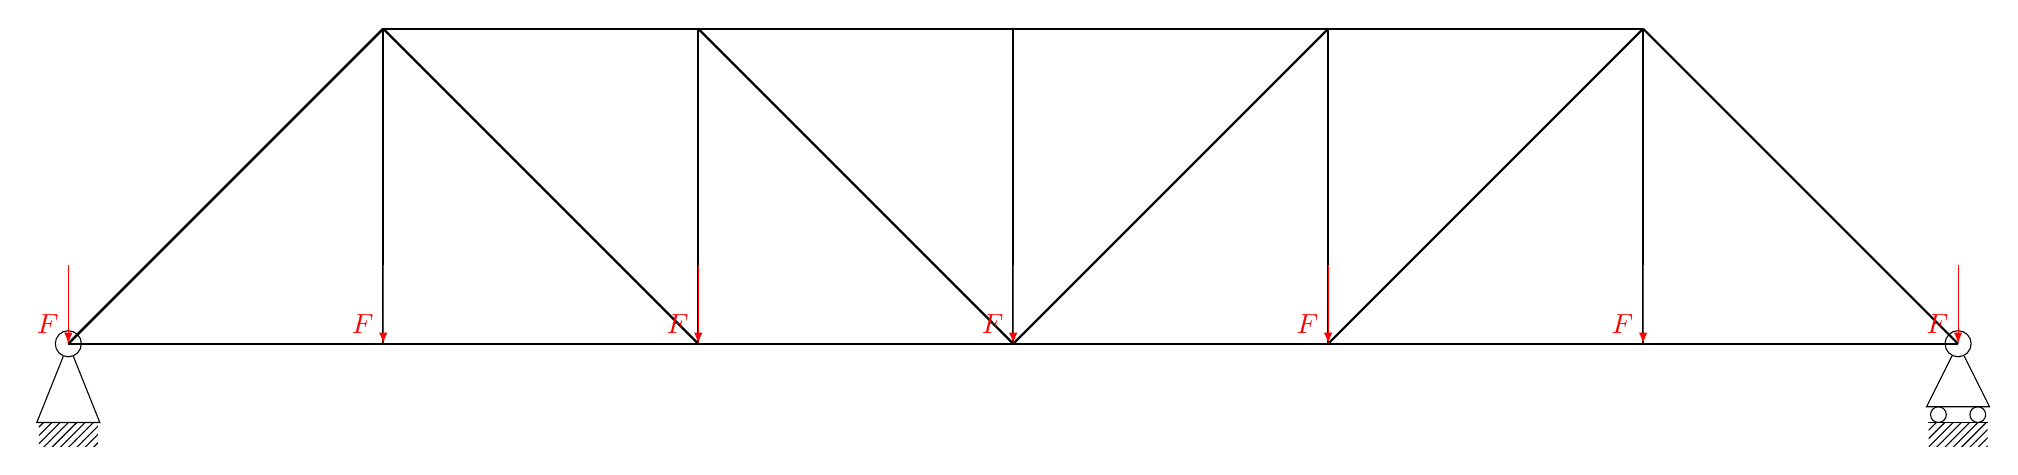
\begin{tikzpicture}[>=latex]
%===DEF. COMPONENTS====
 \def\carrello(#1,#2,#3){
 \begin{scope}[shift={(#1,#2)}]
 \node[draw,circle,fill=#3,minimum width=0.01cm] (S) at (0,0){};
 \draw (S) -- (-0.4,-0.8) -- (+0.4,-0.8) -- (S);
 \draw (0.25,-0.9) circle[radius = 0.1];
 \draw (-0.25,-0.9) circle[radius = 0.1];
 \node (g1) at (0,-1) [ground,anchor=north]{};
 \draw (g1.north west) -- (g1.north east);
 \end{scope}
}

\def\cerniera(#1,#2,#3){
 \begin{scope}[shift={(#1,#2)}]
 \node[draw,circle,fill=#3,minimum width=0.01cm] (S) at (0,0){};
 \draw (S) -- (-0.4,-1) -- (+0.4,-1) -- (S);
 \node (g1) at (0,-1) [ground,anchor=north]{};
 \draw (g1.north west) -- (g1.north east);
 \end{scope}
}
%===2D Frame===
\tikzset{ground/.style ={fill, pattern = north east lines, draw = none, minimum width = 0.75cm, minimum height = 0.3cm}}
%===scheme struct=====
\coordinate (a) at (0,0);
\coordinate (b)	at (4,0);
\coordinate (c) at (8,0);
\coordinate (d) at (12,0);
\coordinate (e) at (16,0);
\coordinate (f) at (20,0);
\coordinate (g) at (24,0);
\coordinate (b1) at (4,4);
\coordinate (c1) at (8,4);
\coordinate (d1) at (12,4);
\coordinate (e1) at (16,4);
\coordinate (f1) at (20,4);
%===orizontal line===
\draw[thick] (a) -- (g);
\draw[thick] (b1) -- (f1);
%===oblicque line===
\draw[thick] (a) -- (b1) ; \draw[thick] (f1) -- (g);
\draw[thick] (c) -- (b1) ; \draw[thick] (e) -- (f1);
\draw[thick] (d) -- (c1) ; \draw[thick] (d) -- (e1);
\draw[thick] (a) -- (b1) ; 
%===vertical line===
\draw[thick] (b) -- (b1); \draw[thick] (c) -- (c1);
\draw[thick] (d) -- (d1); \draw[thick] (e) -- (e1); 
\draw[thick] (f) -- (f1);
%===constraint===
\carrello(24,0,none)
\cerniera(0,0,none)
%===force===  
\coordinate (fmy) at ($(a) + (0,1)$);  
\draw[red,->] (fmy) -- (a) node[pos=1, above left] {$F$};
\coordinate (fmy) at ($(b) + (0,1)$); 
\draw[red,->] (fmy) -- (b) node[pos=1, above left] {$F$};
\coordinate (fmy) at ($(c) + (0,1)$); 
\draw[red,->] (fmy) -- (c) node[pos=1, above left] {$F$};
\coordinate (fmy) at ($(d) + (0,1)$);  
\draw[red,->] (fmy) -- (d) node[pos=1, above left] {$F$};
\coordinate (fmy) at ($(e) + (0,1)$); 
\draw[red,->] (fmy) -- (e) node[pos=1, above left] {$F$};
\coordinate (fmy) at ($(f) + (0,1)$); 
\draw[red,->] (fmy) -- (f) node[pos=1, above left] {$F$};
\coordinate (fmy) at ($(g) + (0,1)$); 
\draw[red,->] (fmy) -- (g) node[pos=1, above left] {$F$};
\end{tikzpicture}}
\caption{Bridge scheme}
\label{img:HW1:Sche}
\end{figure}
%========================================
\noindent To fix the problem, we started the construction of the model building nodes and subsequently connected with \emph{"truss"} elements, come the results shows in the figure \ref{img:HW1-modelGeom}.
Constraints to the bridge ends were added as requested by the problem. A distributed force was applied along the length of the two bays.
Later it was used the same model to analyze the second question.
\begin{figure}[!h]
\centering
\includegraphics[width=0.8\linewidth]{imgHW1/GeometryLoad}
\caption{Model loaded and bound structure}
\label{img:HW1-modelGeom}
\end{figure}
\section{Result}
\subsection{Problem 1}
In the post processing simulation results are observed in the figures \ref{img:HW1-AxialForce} and \ref{img:HW1-AxialStress}, where you can observe the distribution of axial forces and the distribution of axial stress respectively.\\
The displacement of the nodes is shown in the figure \ref{img:HW1-Displacement}, where it is possible to observe that the maximum displacement is obtained in the vicinity of the nodes and is equal to $62,7759 \, mm$.
\begin{figure}[!h]
\centering %centrata
\includegraphics[width=0.8\linewidth]{imgHW1/AxialForce}
\caption{Distibution of axial force}
\label{img:HW1-AxialForce}
\end{figure}
\begin{figure}[!h]
\centering %centrata
\includegraphics[width=0.8\linewidth]{imgHW1/AxialStress}
\caption{Distibution of axial stress}
\label{img:HW1-AxialStress}
\end{figure}
\begin{figure}[!h]
\centering %centrata
\includegraphics[width=0.8\linewidth]{imgHW1/Displacement}
\caption{Displacement of the structure}
\label{img:HW1-Displacement}
\end{figure}\pagebreak\\
\subsection{Problem 2}
For the second question we have used the command \textsc{\emph{NMODIF}} as required to change the position of the nodes by varying the height in order to obtain the minimum deflection of the structure. It has been avoided during the execution of the loop, all those configurations like "M" shape.
\begin{table}[h]
\centering
\footnotesize
\begin{tabular}{ccccccc}
\hline
Number	  & 					  &					  &deflaction & deflaction & deflaction\\
interaction & $\Delta y1$ & $\Delta y2$ &  node 15    &  node 16  & node 17\\
				  &					  &					  & [mm]       & [mm]       & [mm]\\
\hline
806 &   7100,00 &   7100,00 &   -29,4321048924 &   -30,9574832350 &   -29,4321048924\\
807 &   7100,00 &   7200,00 &   -29,2877380752 &   -30,3744253498 &   -29,2877380752\\
808 &   7100,00 &   7300,00 &   -29,1891942493 &   -29,8702541041 &   -29,1891942493\\
809 &   7100,00 &   7400,00 &   -29,1335772891 &   -29,4401993777 &   -29,1335772891\\
\color{red}810 &\color{red}   7100,00 &\color{red}   7500,00 & \color{red}  -29,1182105600 &  \color{red} -29,0798440735 &\color{red}   -29,1182105600\\
811 &   7100,00 &   7600,00 &   -29,1406179070 &   -28,7850939406 &   -29,1406179070\\
812 &   7100,00 &   7700,00 &   -29,1985064925 &   -28,5521503107 &   -29,1985064925\\
813 &   7100,00 &   7800,00 &   -29,2897512823 &   -28,3774854310 &   -29,2897512823\\
814 &   7100,00 &   7900,00 &   -29,4123810029 &   -28,2578201188 &   -29,4123810029\\
815 &   7100,00 &   8000,00 &   -29,5645654149 &   -28,1901034907 &   -29,5645654149\\
\hline
\end{tabular}
\caption{Displacement of bridge}
\label{tab:WH1-Disp}
\end{table}\\\pagebreak
\newpage
\noindent In the graph \ref{img:1-Disp} is observable the needed results of the iterations, we obtain by moving nodes of a value equal to $\Delta y1 = 3100 \, mm$ to the node 15 and 17 and an increase equal to $\Delta y2 = 3500 \, mm$ to the node 15.\\
\noindent The configuration of the structure with minimum deflection is observable in Figure \ref{fig:HW1-nodemod} where the displacement is equal to $31,6387 \, mm$.
\begin{figure}[h]
\centering
\begin{tikzpicture}
\pgfplotsset{cycle list={cyan\\purple\\},major grid style={dashed},}
\begin{axis}[
					width=15cm,
					height=9cm,
 					 xmin=-10, xmax=1000,
        			ymin=-90, ymax=0,
					grid=major,
					xlabel=Iteration number,
					ylabel=Deflection $mm$]
\addplot table[smooth,mark=none, y=def1, x=n]{data.dat};
\addlegendentry{deflection node 15}
\addplot table [smooth,mark=none, y=def2, x=n]{data.dat};
\addlegendentry{deflection node 16}
\addplot[mark=none, black,domain=-10:810, samples=2, dash dot]
 {-29.11821056};
\draw [dash dot](axis cs:810,-90) -- (axis cs:810,-29.11821056) node [above] {
\textsc{\tiny \color{red}min deflection}};
\end{axis}
\end{tikzpicture}
%===Zoom===========================
\begin{tikzpicture}
\pgfplotsset{cycle list={cyan\\purple\\},major grid style={dashed},}
\begin{axis}[
						width=15cm,
						height=5cm,
 						xmin=800, xmax=900,
        				ymin=-35, ymax=-20,
						grid=major,
						xlabel= Iteration number,
						ylabel= Deflection $mm$]
\addplot table[smooth,mark=none, y=def1, x=n]{data.dat};
\addlegendentry{deflection node 15}
\addplot table [smooth,mark=none, y=def2, x=n]{data.dat};
\addlegendentry{deflection node 16}
\addplot[mark=none, black,domain=-10:810, samples=2, dash dot]
 {-29.11821056};
\draw [dash dot](axis cs:810,-90) -- (axis cs:810,-29.11821056) node [above] {
\textsc{\tiny \color{red}min deflection}};
\end{axis}
\end{tikzpicture}
\caption{Displacement of bridge}
\label{img:1-Disp}
\end{figure}
\begin{figure}[h]
\centering
\includegraphics[width=0.8\linewidth]{imgHW1/Displacement-modifyA810}
\caption{minimum deflaction}
\label{fig:HW1-nodemod}
\end{figure}
\section{Command list}
\begin{multicols}{2}
\scriptsize
\lstinputlisting[language=APDL, style=apdl-modified]{CommandListHW1.txt}
\normalsize
\end{multicols}
	\chapter{Homework 2}
\section{Introduction}
Using beam elements, build up a FE model of the hook shown in the Figure. Determine the
maximum displacement, the maximum bending stress, shear and bending moment diagrams. Compare the results obtained considering the cross-sections 1 and 2 shown
below. Discuss the need of mesh refinement.\\
\noindent Data:\\
$F = 20 \, kN \quad E = 205 \, GPa \quad \upsilon=0.3$\\
\begin{figure}[!h]
\centering
\subfloat{\includegraphics[width=.30\textwidth]{/imgHW2/HW2}} \quad
\subfloat{\includegraphics[width=.45\textwidth]{/imgHW2/HW2-1}} 
\end{figure}
\section{Approach the problem}
For this problem we are first costritute the two custom cross sections, in the figures \ref{img:HW2-KeySection}, \ref{img:HW2-AREASection} and \ref{img:HW2-MeshSection}; can be observed the construction phases then a free mesh is applied to both stat and saved in their respective files.
\begin{figure}[!h]
\centering
\subfloat[][Section 1\label{img:HW2_KEYsec1}]{\includegraphics[width=.65\linewidth]{imgHW2/Part1/KEYPOINT-SEC1}}\,
\subfloat[][Section 2\label{img:HW2_KEYsec2}]{\includegraphics[width=.65\linewidth]{imgHW2/Part2/KEYPOINT-SEC2}}
\caption{Keyponit Section}
\label{img:HW2-KeySection}
\end{figure}
\begin{figure}[!h]
\centering
\subfloat[][Section 1\label{img:HW2_GEOMsec1}]{\includegraphics[width=.8\linewidth]{imgHW2/Part1/GEOM-SEC1}}\,
\subfloat[][Section 2\label{img:HW2_GEOMsec2}]{\includegraphics[width=.8\linewidth]{imgHW2/Part2/GEOM-SEC2}}
\caption{Geometry of sections}
\label{img:HW2-GeomSection}
\end{figure}
\begin{figure}[!h]
\centering
\subfloat[][Section 1\label{img:HW2_AREAsec1}]{\includegraphics[width=.8\linewidth]{imgHW2/Part1/AREA-SEC1}}\,
\subfloat[][Section 2\label{img:HW2_AREAsec2}]{\includegraphics[width=.8\linewidth]{imgHW2/Part2/AREA-SEC2}}
\caption{Area of sections}
\label{img:HW2-AREASection}
\end{figure}
\pagebreak\\
\begin{figure}[!h]
\centering
\subfloat[][Section 1\label{img:HW2_sec1}]{\includegraphics[width=.8\linewidth]{imgHW2/Part1/MESH-SEC1}}\,
\subfloat[][Section 2\label{img:HW2_sec2}]{\includegraphics[width=.8\linewidth]{imgHW2/Part2/MESH-SEC2}}
\caption{Meshed Section}
\label{img:HW2-MeshSection}
\end{figure}\noindent
In this case it is defined the geometry of the hook through the use of \emph{keypoints} and subsequently connected by lines, as ahow in fiugure \ref{img:HW2-Geometry}.
Then the mesh using the section $n^{\circ}$1 was created in the previuos step and then the section $n^{\circ}$2.\\
For the section $n^{\circ} 1$ the result in figure \ref{img:HW2_sec1}, while section $n^{\circ} 2$ in picture \ref{img:HW2_sec2}.
\begin{figure}[!h]
\centering 
\subfloat[][Keypoint]{\includegraphics[width=.8\linewidth]{imgHW2/Part1/Keypoint-SEC1-mm-4}}\,
\subfloat[][Full geometry]{\includegraphics[width=.8\linewidth]{imgHW2/Part2/GEOM-SEC2-mm-4}}
\caption{Geometry's hook}
\label{img:HW2-Geometry}
\end{figure}
\begin{figure}[!h]
\centering 
\subfloat[][Section 1]{\includegraphics[width=.8\linewidth]{imgHW2/Part1/FORCE-SEC1-mm-4}}\,
\subfloat[][Section 2]{\includegraphics[width=.8\linewidth]{imgHW2/Part2/FORCE-SEC2-mm-4}}
\caption{Hook meshed and costraint}
\label{img:HW2-Mesh+Costraint}
\end{figure}
\section{Result}
In conclusion is shown in the table of performance comparison of the two cross section.\\
\begin{table}[!h]
\centering
\begin{tabular}{lcccc}
\hline
       Area  	& Displacement & maximum bending stress	 & minimum bending stress\\
    $mm^2$ &	 $mm$			& $MPa$				& $MPa$\\
\hline
       	1000	&	2,59533		&283,82				&-324,366\\
\hline
\end{tabular}
\caption{Recap section 1}
\label{table:HW2:RecapSec1}
\end{table}
\begin{table}[!h]
\centering
\begin{tabular}{cccc}
\hline
       Area  & Displacement 	& maximum 	bending stress	& minimum bending stress\\
    $mm^2$ &	 $mm$			& $MPa$				& $MPa$\\
\hline
    658,84	&	2,8004			&	318,819			&	-318,819\\
\hline
\end{tabular}
\caption{Recap section 2}
\label{table:HW2:RecapSec2}
\end{table}
\begin{enumerate}
\item It is observed in the first section a greater deformation despite the area is larger in size when compared with the second.
\item Whereas the difference in the area of the sections, the displacement of the section 2 is similar to the first.
\item Section 2 does not show differences in the stress since Section 1.
\end{enumerate}
In conclusion it is observed a better performance of the section 2 to equal forces applied.
Subsequently, the analysis is repeated increased the division into examination number generating, therefore, a more dense mesh from which it is observed that the obtained have results are very close, in the table \ref{tab:HW2-ref1}, \ref{tab:HW2-ref2}.
\begin{table}[!h]
\centering

\begin{tabular}{ccccc}
\hline
size 	& section	& Bending Stress min 	&	bending stress max	&	displacement\\
		&			& $MPa$					& 	$MPa$				& $mm$\\
\hline
1		&	1		&-324,327				&	283,786				&	2,59533\\
4		&	1		&-324,366				&	283,82				&	2,59533\\
7		&	1  		& -324,45				&	283,894				&	2,59533\\
10		&	1		&-324,584				&	284,011				&	2,59533\\
16		&	1		&-324,989				&	284,365				&	2,59533\\
22		&	1		&-325,36				&	284,69				&	2,59533\\
\hline
\end{tabular}

\caption{Sensibility result to mesh refiniment}
\label{tab:HW2-ref1}
\end{table}
\begin{table}[!h]
\centering
\begin{tabular}{ccccc}
\hline
size 	& section	& Bending Stress min 	&	bending stress max	&	displacement\\
		&			& $MPa$					& 	$MPa$				& $mm$\\
\hline
1		&	2		&	-318,78				&	318,78				&	2,8004\\
4		&	2		&	-318,819			&	318,819				&	2,8004\\
7		&	2  		&	-318,901			&	318,901				&	2,8004\\
10		&	2		&	-319,033			&	319,033				&	2,8004\\
16		&	2		&	-319,431			&	319,431				&	2,8004\\
22		&	2		&	-319,796			&	319,796				&	2,8004\\
\hline
\end{tabular}
\caption{Sensibility result to mesh refiniment}
\label{tab:HW2-ref2}
\end{table}
\pagebreak\\
The following pictures shows the results obtained from the simulation.
\begin{figure}[!h]
\centering
\subfloat[][Section 1]{\includegraphics[width=.65\linewidth]{imgHW2/Part1/Displacemt-SEC1-mm-4}}\,
\subfloat[][Section 2]{\includegraphics[width=.65\linewidth]{imgHW2/Part2/Displacemt-SEC2-mm-4}}
\label{img:HW2-Displacemt}
\caption{Result Displacement diagram}
\end{figure}
\begin{figure}[!h]
\centering 
\subfloat[][Section 1]{\includegraphics[width=.8\linewidth]{imgHW2/Part1/NODALSOLUTION-SEC1-mm-4}}\,
\subfloat[][Section 2]{\includegraphics[width=.8\linewidth]{imgHW2/Part2/NODALSOLUTION-SEC2-mm-4}}
\label{img:HW2-NodalSolu}
\caption{Result nodal solution diagram}
\end{figure}
\begin{figure}[!h]
\centering 
\subfloat[][Section 1]{\includegraphics[width=.8\linewidth]{imgHW2/Part1/BENDINMAX-SEC1-mm-4}}\,
\subfloat[][Section 2]{\includegraphics[width=.8\linewidth]{imgHW2/Part2/BENDINMAX-SEC2-mm-4}}
\label{img:HW2-bendingmax}
\caption{Result max bending diagram}
\end{figure}
\begin{figure}[!h]
\centering 
\subfloat[][Section 1]{\includegraphics[width=.8\linewidth]{imgHW2/Part1/BENDINGMIN-SEC1-mm-4}}\,
\subfloat[][Section 2]{\includegraphics[width=.8\linewidth]{imgHW2/Part2/BENDINGMIN-SEC2-mm-4}}
\label{img:HW2-bendingmin}
\caption{Result minimum bending stress diagram}
\end{figure}
\begin{figure}[!h]
\centering 
\subfloat[][Section 1]{\includegraphics[width=.8\linewidth]{imgHW2/Part1/MOMENT-SEC1-mm-4}}\,
\subfloat[][Section 1]{\includegraphics[width=.8\linewidth]{imgHW2/Part1/MOMENT-SEC1-mm-4}}
\label{img:HW2-Moment}
\caption{Result Moment diagram}
\end{figure}
\begin{figure}[!h]
\centering
\subfloat[][Section 1]{\includegraphics[width=.8\linewidth]{imgHW2/Part1/SHEAR-SEC1-mm-4}}\,
\subfloat[][Section 2]{\includegraphics[width=.8\linewidth]{imgHW2/Part2/SHEAR-SEC2-mm-4}}
\label{img:HW2-Shear}
\caption{Result shear diagram}
\end{figure}
\section{Command list}
\begin{multicols}{2}
\scriptsize
\lstinputlisting[language=APDL, style=apdl-modified]{CListHW2-Sec1.txt}
\lstinputlisting[language=APDL, style=apdl-modified]{CListHW2-Sec2.txt}
\lstinputlisting[language=APDL, style=apdl-modified]{CommandListHW2-SEC1.txt}
\normalsize
\end{multicols}
	\chapter{Homework 3}
\begin{minipage}{.70\textwidth}
\centering
\includegraphics[width=0.8\linewidth]{imgHW3/HW3}
\end{minipage}
\begin{minipage}{.70\textwidth}
\begin{tabular}{l}
        DATA:\\
        $\frac{D}{d} = 1.4 $\\
        $\frac{r}{d} = \frac{1}{20} $\\
        $R = \frac{(D-d)}{2}$\\
        Material: steel
\end{tabular}
\end{minipage}\\\\
The figure illustrates a shouldered shaft carrying a relief groove to reduce the notch stress concentration effect. The shaft is subject to an axial load F. Using axisymmetric plane elements, build up a FE model that allows:
\begin{enumerate}
\item determining the stress concentration factor in the absence of the relief groove. Carry out a convergence analysis and compare the obtained result with solutions available in the literature.
\item determining the stress concentration factor as a function of the non-dimensional position x of the relief groove. Try to identify an optimal position. Use a mesh refinement level similar to that obtained in the convergence analysis carried out in point 1).\\
The stress concentration factor is defined as:
$Kt = \sigma_{1,max};\, \sigma_{1,max}$: maximum first principal stress in the model; $S_{net} = \frac{F}{\frac{\pi}{4}d^2}$.\\
 It is required to create a mapped mesh at least in the neighbourhood of the fillets of the shoulder and at the groove. Pay attetion to avoid distorted elements. Apply the axial force as a uniformly distributed pressure.
 \end{enumerate}
\section{Approach the problem}
For this problem we have adopted element type \emph{\textsc{Plane182}} for the problem without relief groove, on the other hand we have adoptd element type \emph{\textsc{Plane183}} for the shaft with relief groove because \textsc{plane183} is well suited to model irregular meshes.\\
The cross section of the shaft is created with axisymmetric elements along the y-direction.\\
A mesh refinement acting along the shoulder surface is made in order to avoid worthless computational costs. 
The main assumption adopted in the resolution of the problem is the choice of the keyoptions.
\begin{itemize}
\item The element technology:
Keyoption(1) = 0 due to the only axial traction of the shaft (no bending moment domination);
\item Structural behavior:
Keyoption(3) =  1 due to the axisymmetry of the problem.
\end{itemize}
The material present the follow proprities:
\begin{itemize}
\item Modulus of elasticity: $210\, GPa$;
\item Poissons ratio $0.3$.
\end{itemize}
The shaft is loaded along the axis $y$ with a distributed force.\\
Finally we set \emph{keyopt} for axisymmetric element behaviour.
The two tree models were constructed by placing the keypoint and then connected by lines, both have sub-divisions in areas to generate the mapped mesh. The groove is a function of the parameter x, the geometric model is observable in the figures \ref{img:HW3-Geometry}, while in subsequent images \ref{img:HW3-mesh}, the mesh model.
\begin{figure}[!h]
\centering
\subfloat[][Shaft without relief groove]{\includegraphics[width=.8\textwidth]{/imgHW3/Part1/HW3-Geometry_PART1}} \,
\subfloat[][Shaft relief groove]{\includegraphics[width=.8\textwidth]{/imgHW3//Part2/HW3-Geometry_PART2}} 
\caption{Geometry Model}
\label{img:HW3-Geometry}
\end{figure}
\begin{figure}[!h]
\centering
\subfloat[][Shaft without relief groove]{\includegraphics[width=.8\textwidth]{/imgHW3/Part1/HW3-Mesh_PART1}} \,
\subfloat[][Shaft relief groove]{\includegraphics[width=.8\textwidth]{/imgHW3//Part2/HW3-Mesh_PART2}}
\caption{Mapped mesh's model}
\label{img:HW3-mesh}
\end{figure}
\section{Result}
The stress concentration factor is defined as:
\[
	K_{t} = \frac{\sigma_{1,Max}}{S_{net}} 
\]
$\sigma_{1,Max}$ is equal to maximum first principal stress in the model:
\[
	S_{net}=\frac{F}{\frac{\pi}{4} d^{2}} = 15000 \, MPa
\]
After analysis of convergence can be observed, in the table \ref{table:HW3-KtWithoutRelief}, that as the number of mesh divisions of the $K_{t}$ value tends to stabilize toward the value $K_{t} \approx 2,4$. On the other hand it is observed that for a bonus multiplier of the divisions\footnote{we have adopte: 
	\begin{tabular}{l}
		n\_div\_a, $3*i$\\ 
		n\_div\_b, $2*i$\\
		n\_div\_c, $3*i$
	\end{tabular}
} 
of $10$ you get a value close to that available in the literature in fact, the theoretical value is approximately equal to $K_{t}=2,3$; show in figure \ref{img:HW3-KtGraph}.\begin{figure}[!h]
\centering
\includegraphics[width=.8\textwidth]{/imgHW3/Kt-Graph}
\caption{stress intensity factor graph}
\label{img:HW3-KtGraph}
\end{figure}\\
\noindent Instead performing a refinement of the mesh in the areas of the fillet it leads to a smaller number of divisions and a comparable number of elements thereby reducing the computational cost.\\
In fact, just a multiplier $4$ to obtain $12$ divisions are needed with a level 1 refinement to obtain a number of elements equal to $788$ and a $K_{t}=2,334$ close to the theoretical value first found, like show in table \ref{table:HW3-KtWithoutReliefREF}.\pagebreak
\begin{table}[t]
\centering
\begin{tabular}{cccc}
 \hline
  multiplier	  &				&	$S1_{max}$\\
  for n. division & n. elements &   $MPa$	&  $K_{t}$\\
 \hline
  24 &      18432 &           37033,121   &            2,469\\
  23 &      16928 &           36953,023   &            2,464\\
  22 &      15488 &           36866,906   &            2,458\\
  21 &      14112 &           36773,375   &            2,452\\
  20 &      12800 &           36671,621   &            2,445\\
  19 &      11552 &           36560,215   &            2,437\\
  18 &      10368 &           36437,992   &            2,429\\
  17 &       9248 &           36303,395   &            2,420\\
  16 &       8192 &           36154,652   &            2,410\\
  15 &       7200 &           35988,516   &            2,399\\
  14 &       6272 &           35802,207   &            2,387\\
  13 &       5408 &           35591,184   &            2,373\\
  12 &       4608 &           35350,777   &            2,357\\
  11 &       3872 &           35073,625   &            2,338\\
  10 &       3200 &           34751,336   &            2,317\\
   9 &       2592 &           34371,125   &            2,291\\
   8 &       2048 &           33916,500   &            2,261\\
   7 &       1568 &           33363,152   &            2,224\\
   6 &       1152 &           32674,590   &            2,178\\
   5 &        800 &           31797,691   &            2,120\\
   4 &        512 &           30636,627   &            2,042\\
   3 &        288 &           29044,623   &            1,936\\
   2 &        128 &           26681,012   &            1,779\\
   1 &         32 &           22991,930   &            1,533\\
 \hline
\end{tabular}
\caption[]{Number of division without refiniment}
\label{table:HW3-KtWithoutRelief}
\end{table}
\noindent In the second part of the problem, where the model with relief grooves, it is set to the same size of the mesh and refinement level of the previous model calculated in the first part of the problem of obtaining a $K_{t}=1,762$ as a function of the dimensionless value \textsc{x} where \textsc{x} = $1,5$.  It can be seen in figure \ref{img:HW3-KtFunc} trends the fly $K_{t}$ as \textsc{x} changes.
\begin{table}[!h]
\centering
\begin{tabular}{cccc}
 \hline
  multiplier	  &				&	$S1_{max}$\\
  for n. division & n. elements &   $MPa$	&  $K_{t}$\\
  \hline
  24 &      19913 &           38378,484     &          2,559\\
  23 &      18346 &           38358,875     &          2,557\\
  22 &      16844 &           38281,844     &          2,552\\
  20 &      14041 &           38218,875     &          2,548\\
  19 &      12729 &           38162,270     &          2,544\\
  18 &      11488 &           38089,398     &          2,539\\
  17 &      10306 &           38068,324     &          2,538\\
  16 &       9189 &           37995,539     &          2,533\\
  15 &       8139 &           37941,855     &          2,529\\
  14 &       7155 &           37834,023     &          2,522\\
  13 &       6226 &           37724,781     &          2,515\\
  12 &       5366 &           37641,707     &          2,509\\
  11 &       4570 &           37510,848     &          2,501\\
  10 &       3836 &           37358,570     &          2,491\\
   9 &       3171 &           37141,441     &          2,476\\
   8 &       2564 &           36991,867     &          2,466\\
   7 &       2024 &           36729,227     &          2,449\\
   6 &       1548 &           36311,852     &          2,421\\
   5 &       1136 &           35868,047     &          2,391\\
   4 &        788 &           35008,906     &          2,334\\
   3 &        504 &           33962,035     &          2,264\\
   2 &        284 &           32086,471     &          2,139\\
   1 &        116 &           29012,170     &          1,934\\
  \hline
\end{tabular}
\caption[]{Number of division with refiniment}
\label{table:HW3-KtWithoutReliefREF}
\end{table}
\begin{figure}[!h]
\centering
\begin{tikzpicture}
\pgfplotsset{cycle list={cyan\\purple\\},major grid style={dashed},}
\begin{axis}[
					ymin = 1.60,
					ymax = 2.2,
					width = 15cm,
					height = 7.5cm,
					grid=major,
					xlabel= Iteration number $x$,
					ylabel= Stress intesitivity factor $K_{t}$]
\addplot table[smooth, Aquamarine, mark=none, y=kt, x=x]{S1max.txt};
\end{axis}
\end{tikzpicture}
\caption{$K_{t}$ function of \textsc{x}}
\label{img:HW3-KtFunc}
\end{figure}
\begin{figure}[!h]
\centering
\subfloat[][Shaft without relief groove]{\includegraphics[width=.8\textwidth]{/imgHW3/Part1/HW3-Displacement_PART1}} \,
\subfloat[][Shaft relief groove]{\includegraphics[width=.8\textwidth]{/imgHW3//Part2/HW3-Displacement_PART2}} 
\caption{Displacement}
\label{img:HW3-displacement}
\end{figure}
\begin{figure}[!h]
\centering
\subfloat[][Shaft without relief groove]{\includegraphics[width=.8\textwidth]{/imgHW3/Part1/HW3-FirstPrincipalStress_PART1}} \,
\subfloat[][Shaft relief groove]{\includegraphics[width=.8\textwidth]{/imgHW3//Part2/HW3-FirstPrincipalStress_PART2}} 
\caption{First Principal Stress}
\label{img:HW3-FirstPrincipalStress}
\end{figure}
%\noindent Mesh without refinement approach is more prevently and involves additional computational costs to reach the same results of the refinement approach. 
%The $K_{t}$ calculated is a bit different from the one available in the literature (2,56  2,2).
%The optimal configuration for shaft with relief groove  among the results is in the proximity of the shoulder %(in this case 6 mm far from the shoulder).
\section{Conclusion}
For the model absence of the relief groove: the analysis without refinement is acceptable,
comparing literature value found on graph $K_{t} \approx 2,3$ and value before found $K_{t}=2,334$, that is acceptable.\\
On the other hand, model with relief groove: the stress concentration decreases with decrease of \textsc{x} coefficient, this behavior is normal for shadow effect, where the stress concentration is minor respect at the case without relief groove.
\section{Command list}
\begin{multicols}{2}
\scriptsize
\lstinputlisting[language=APDL, style=apdl-modified]{CommandList-HW3.txt}
\lstinputlisting[language=APDL, style=apdl-modified]{CommandList-HW3Part2.txt}
\normalsize
\end{multicols}
	\chapter{Homework 4}
\begin{minipage}{.70\textwidth}
\centering
\includegraphics[width=0.8\linewidth]{imgHW4/HW4}
\end{minipage}
\begin{minipage}{.70\textwidth}
\begin{tabular}{l}
        DATA:\\
        Material: steel;\\
        Pressure: $P_{i}= 10$ \textsc{bar};
\end{tabular}
\end{minipage}\\\\
The figure illustrates a T pipe connector to be used in a hydraulic circuit subject to internal pressure $p_{i}$. Using shell elements and taking into account the symmetry, build up a FE model composed of a mapped mesh that allows:
\begin{enumerate}
\item determining (meridional and circumferential) membrane stresses far from the junction between the two pipes;
\item determining membrane and bending stress distribution along the periphery of the pipes' junction.
\end{enumerate}
\section{Approach the problem}
the elements that compose the structure: are used in three-dimensional shell elements, \textsc{shell181}, having the thickness of the two tubes are first defined. The stress analysis will be conducted on the inner surface and the average plane of the elements.
You create keypoint, connect via lines and generating areas for extrusion lines, 
two local references are defined with cylindrical cooordinate to carry out these operations, as show in figure \ref{img:HW4_GEOMsec1}.
To realize the junction intersected areas that make up the two tubes and the excess arising from its construction have been eliminated. At this point the areas that compose the model are divided into smaller areas in the vicinity of the junction. This is done later to create a denser mesh in this area.
The result that is obtained is the following \ref{img:HW4_GEOMsec3}.
\begin{figure}[!h]
\centering
\subfloat[][First step construnction\label{img:HW4_GEOMsec1}]{\includegraphics[width=.7\linewidth]{imgHW4/HW4-Geometry_1}}\,
\subfloat[][Second step construction\label{img:HW4_GEOMsec3}]{\includegraphics[width=.7\linewidth]{imgHW4/HW4-Geometry_3}}
\caption{Geometry of T pipe}
\label{img:HW4-GeomSection}
\end{figure}
\pagebreak\\
To realize the mesh are divided all components then mesh mapped areas, show in frame \ref{img:HW4_Mesh}. Particular attention taken into accoutn at zone of junction, result show in \ref{img:HW4_MeshDetail}.\\
Once sure that the unit vectors normal to the shell elements have always the same direction, fig. \ref{img:HW4-NormSurf}, apply the symmetry constraints and internal pressure. \\They then analyze two different way:
\begin{itemize}
\item It sets to 0 the displacement in the y direction of a node: the constraints on symmetry in fact, they do not eliminate this degree of freedom. It could be a rigid translation of the component;
\item they are binding on the long-x node displacements in the flow line (line used to extrude the tube) because it is assumed that the tube can be extended in this direction. Is done the same for the vertical pipe, then set to zero along the y displacement of the nodes present on the line. In this way also avoids the rigid translation of the model.
\end{itemize}
At this point it solves the structure and proceed with the analysis of the results.
\begin{figure}[!h]
\centering
\includegraphics[width=.8\linewidth]{imgHW4/HW4-Mesh}
\caption{Meshed model}
\label{img:HW4_Mesh}
\end{figure}
\begin{figure}[!h]
\centering
\includegraphics[width=.8\linewidth]{imgHW4/HW4-Mesh-Zoom}
\caption{Detail of the mesh to the pipe joint }
\label{img:HW4_MeshDetail}
\end{figure}
\begin{figure}[h]
\centering
\includegraphics[width=0.8\linewidth]{imgHW4/HW4-NormSurf}
\caption{Vector normal to surface}
\label{img:HW4-NormSurf}
\end{figure}\\
\pagebreak
\section{Result}
The membrane stress are visible in \ref{img:HW4_SX1} and \ref{img:HW4_SY1},
it is noted that at a certain distance from the junction of the membrane stress assume nearly costant value and the flexural value close to zero. It then sees that in the proximity of junction of the flexural stress become important and are obtained for very high value of stress.
Regarding the convergence of the solution, it can be seen that going to densify the mesh the value of the stress on the junction does not converge as this area subject to a strucutral singlularity.
\begin{figure}[!h]
\centering
\subfloat[][Full view \label{img:HW4_SX1}]{\includegraphics[width=.7\linewidth]{imgHW4/HW4-SolutionSX}}\,
\subfloat[][Detail at junction \label{img:HW4_SX1zoom}]{\includegraphics[width=.7\linewidth]{imgHW4/HW4-SolutionSX-Zoom}}
\caption{Membrane meridional stress}
\label{img:HW4-SX}
\end{figure}
\begin{figure}[!h]
\centering
\subfloat[][Full view \label{img:HW4_SY1}]{\includegraphics[width=.8\linewidth]{imgHW4/HW4-SolutionSY}}\,
\subfloat[][Detail at junction\label{img:HW4_SY1zoom}]{\includegraphics[width=.8\linewidth]{imgHW4/HW4-SolutionSY-Zoom}}
\caption{Membrane circumferential stress}
\label{img:HW4-SY}
\end{figure}\\\pagebreak
\newpage
\noindent It then conducted a more detailed analysis going to represent on a graph the progress of efforts along the axial direction of the two tubes, starting from the most distant areas from the junction until you get near it, the result obtained are show in graphs \ref{img:HW4-StressVerticalPipe} for vertical pipe and \ref{img:HW4-StressHorizontalPipe} for horizontal pipe.
\begin{figure}[!h]
\centering
    \resizebox{.8\linewidth}{!}{%\begin{tikzpicture}
%\pgfplotsset{cycle list={blue\\}, major grid style={dashed},}
%\begin{axis}[
%						legend pos=south east,
%						width=15cm,
%						height=10cm,
%        				grid=major,
%        				ylabel=Stress $MPa$,
%        				xlabel=Radius $mm$]
%\addplot [thick, blue, smooth, mark=none] table[y={sx}]{StressVerticalPipe.txt};
%\addlegendentry{Meridional stress}
%\addplot [thick, red, smooth, mark=none] table[y={sy}]{StressVerticalPipe.txt};
%\addlegendentry{Circumferential stress}
%\end{axis}
%\end{tikzpicture}

\begin{tikzpicture}
\pgfplotsset{major grid style={dashed},}
\begin{axis}[
						%legend pos=south east,
						legend cell align={left},
						width=15cm,
						height=10cm,
        				grid=major,
        				ylabel=Stress $MPa$,
        				xlabel=Distance $mm$]
\addplot [thick, NavyBlue, smooth, mark=none] table[y={sx}]  {VerticalStress2.txt};
\addlegendentry{membrane circumferential efforts}
\addplot [thick, Dandelion, smooth, mark=none] table[y={sy}]  {VerticalStress2.txt};
\addlegendentry{meridional membrane efforts}
\addplot [thick, ForestGreen, smooth, mark=none] table[y={sxb}]{VerticalStress2.txt};
\addlegendentry{efforts circumferential flexural}
\addplot [thick, RubineRed, smooth, mark=none] table[y={syb}]{VerticalStress2.txt};
\addlegendentry{meridional efforts flexural}
\addplot [thick, NavyBlue, smooth, mark=none] table[y={sx}]  {VerticalStress1.txt};
\addplot [thick, Dandelion, smooth, mark=none] table[y={sy}]  {VerticalStress1.txt};
\addplot [thick, ForestGreen, smooth, mark=none] table[y={sxb}]{VerticalStress1.txt};
\addplot [thick, RubineRed, smooth, mark=none] table[y={syb}]{VerticalStress1.txt};
\end{axis}
\end{tikzpicture}}
    \caption{Stress vertical pipe}
    \label{img:HW4-StressVerticalPipe}
\end{figure}
\begin{figure}[!h]
\centering
    \resizebox{.8\linewidth}{!}{%\begin{tikzpicture}
%\pgfplotsset{cycle list={blue\\}, major grid style={dashed},}
%\begin{axis}[
%						legend pos=south east,
%						width=15cm,
%						height=10cm,
%        				grid=major,
%        				ylabel=Stress $MPa$,
%        				xlabel=Radius $mm$]
%\addplot [thick, BurntOrange, smooth, mark=none] table[y={sx}]{StressHorizzontalPipe.txt};
%\addlegendentry{Meridional stress}
%\addplot [thick, NavyBlue, smooth, mark=none] table[y={sy}]{StressHorizzontalPipe.txt};
%\addlegendentry{Circumferential stress}
%\end{axis}
%\end{tikzpicture}

\begin{tikzpicture}
\pgfplotsset{major grid style={dashed},}
\begin{axis}[
						%legend pos=south east,
						legend cell align={left},
						width=15cm,
						height=10cm,
        				grid=major,
        				ylabel=Stress $MPa$,
        				xlabel=Distance $mm$]
\addplot [thick, NavyBlue, smooth, mark=none] table[y={sx}]   {HorizzontalStress1.txt};
\addlegendentry{membrane circumferential efforts}
\addplot [thick, Dandelion,smooth, mark=none] table[y={sy}]   {HorizzontalStress1.txt};
\addlegendentry{meridional membrane efforts}
\addplot [thick, ForestGreen, smooth, mark=none] table[y={sxb}]{HorizzontalStress1.txt};
\addlegendentry{efforts circumferential flexural}
\addplot [thick, RubineRed, smooth, mark=none] table[y={syb}]{HorizzontalStress1.txt};
\addlegendentry{meridional efforts flexural}
\addplot [thick, NavyBlue, smooth, mark=none] table[y={sx}]  {HorizzontalStress2.txt};
\addplot [thick, Dandelion, smooth, mark=none] table[y={sy}]  {HorizzontalStress2.txt};
\addplot [thick, ForestGreen, smooth, mark=none] table[y={sxb}]{HorizzontalStress2.txt};
\addplot [thick, RubineRed, smooth, mark=none] table[y={syb}]{HorizzontalStress2.txt};
\end{axis}
\end{tikzpicture}
}
    \caption{Stress horizontal pipe}
    \label{img:HW4-StressHorizontalPipe}
\end{figure}
\section{Conclusion}
The obtained results confirm what was found earlier: the flexural stresses are very low away from the junction and become higher in the vicinity of it; the membrane efforts are constant along the tube and, as regards those circumferential, assume very high values on the junction.
\section{Command list}
\begin{multicols}{2}
\tiny
\lstinputlisting[language=APDL, style=apdl-modified]{CommandList-HW4.txt}
\normalsize
\end{multicols}
	\chapter{Homework 5}
\begin{minipage}{.70\textwidth}
\centering
\includegraphics[width=0.8\linewidth]{imgHW5/HW5}
\end{minipage}
\begin{minipage}{.70\textwidth}
\begin{tabular}{l}
        DATA:\\
        Material: steel;\\
        Pressure: $P_{i}= 10$ \textsc{bar};
\end{tabular}
\end{minipage}\\\\
The T pipe connector analyzed in HW 4 is now filletted at the junction between the two pipes to reduce the stress concentration factor. Using brick elements, build a submodel able to estimate the stress distribution along the periphery of the pipes' junction on the base of the displacement field computed with the shell model developed in HW 4. It is required to:
\begin{enumerate}
\item check for the sensitivity of the results upon the location of the cutting boundaries of the submodel.
\end{enumerate}
\section{Approach the problem}
For this problem, first designing the pattern seen in homework 4 saving the results and after that we realize the submodel.
Using the same work surfaces extrude the two vertical and horizontal cylinders, then they eliminate unneeded volumes. The result as show in figure \ref{img:HW5_GEOMsec1}.
It builds the fillet eliminating the junction that was present in the previous step, figure \ref{img:HW5_GEOMsec3}.
\begin{figure}[!h]
\centering
\subfloat[][First step construnction\label{img:HW5_GEOMsec1}]{\includegraphics[width=.8\linewidth]{imgHW5/HW5-Geometry_1_0}}\,
\subfloat[][Second step construction\label{img:HW5_GEOMsec3}]{\includegraphics[width=.8\linewidth]{imgHW5/HW5-Geometry_2_0}}
\caption{3D Geometry of T pipe}
\label{img:HW5-GeomSection}
\end{figure}\\
The model is now trimmed to the sub pattern using two planes: one through the vertical plane; the second is horizontal. Finally the separate volumes are united in a single body.
It realizes a free mesh with type elements \textsc{solid186}, assigned size of the elements is equal one millimeter; such as to ensure that there are at least two elements in the smallest thickness that makes up the vertical cylinder, the result is observable in fig. \ref{img:HW5_Mesh}.
\begin{figure}[!h]
\centering
\includegraphics[width=.8\linewidth]{imgHW5/HW5-MeshDeatil_1_125}
\caption{Mesh model}
\label{img:HW5_Mesh}
\end{figure}\\
At this point, saving the coordinates of the nodes that are located on the surfaces generated from pattern cutting, for later use to define the conditions of the problem outline. 
The results solution's Homework 4 are recalled and through interpolation is assigned a shift on the nodes that you have saved the coordinates above. Finally applies the same pressure of 10 \textsc{bar} and constraints.
\section{Result}
The study is carried out by varying the distance of the cut boundaries in such a way as not to modify the structure of the problem. defining a sub small model and then increase its size. The analysis is summarized, in the table \ref{tab:HW5_iter}, where the cutting distances are quoted with respect to the junction.\\
\begin{table}[htb]
\centering
\begin{tabular}{cccc}
\hline
       iter&   Vertical cut  boundaries  &     Radius cut boundaries\\ 
       		 &		$mm$                          &       $mm$\\     
\hline
        1	&		30,0000   &    65,0000\\
        2	&    	35,0000   &    70,0000\\
        3 &   	40,0000   &    75,0000\\
        4 &    	45,0000   &    80,0000\\
        5 &    	50,0000   &    85,0000\\
        6 &    	55,0000   &    90,0000\\
\hline
\end{tabular}
\caption{Cut boundaries distance}
\label{tab:HW5_iter}
\end{table}
\newpage
\noindent The results satisfied the equivalent stress, according to Von Mises, obtained under varying cut boundaries are shown in figures \ref{img:HW5-StressEQV_1}, \ref{img:HW5-StressEQV_2} and \ref{img:HW5-StressEQV_3}, it referred to as the stress shifts from the cut boundaries to the fillet.
\begin{figure}[!h]
\centering
\subfloat[][\scriptsize Submodel at cut boundaries $65\,mm$, $65\,mm$\label{img:HW5_StressEqv_0}]{\includegraphics[width=.45\linewidth]{imgHW5/HW5-SolutionEQV_0}}\,
\subfloat[][\scriptsize Submodel at cut boundaries $70\,mm$, $67,50\,mm$\label{img:HW5_StressEqv_25}]{\includegraphics[width=.45\linewidth]{imgHW5/HW5-SolutionEQV_25}}
\caption{Von Mises equivalent stress}
\label{img:HW5-StressEQV_1}
\end{figure}
\begin{figure}[!h]
\centering
\subfloat[][\scriptsize Submodel at cut boundaries $75\,mm$, $70\,mm$\label{img:HW5_StressEqv_50}]{\includegraphics[width=.45\linewidth]{imgHW5/HW5-SolutionEQV_50}}\,
\subfloat[][\scriptsize Submodel at cut boundaries $80\,mm$, $72,50\,mm$\label{img:HW5_StressEqv_75}]{\includegraphics[width=.45\linewidth]{imgHW5/HW5-SolutionEQV_75}}
\caption{Von Mises equivalent stress}
\label{img:HW5-StressEQV_2}
\end{figure}
\begin{figure}[!h]
\centering
\subfloat[][\scriptsize Submodel at cut boundaries $85\,mm$, $75\,mm$\label{img:HW5_StressEqv_100}]{\includegraphics[width=.45\linewidth]{imgHW5/HW5-SolutionEQV_100}}\,
\subfloat[][\scriptsize Submodel at cut boundaries $90\,mm$, $77,50\,mm$\label{img:HW5_StressEqv_125}]{\includegraphics[width=.45\linewidth]{imgHW5/HW5-SolutionEQV_125}}
\caption{Von Mises equivalent stress}
\label{img:HW5-StressEQV_3}
\end{figure}
\newpage
\noindent It is observed in the graph, in the figure \ref{img:HW5-StressSensit}, which initially stress is high, then it takes on a downward path until it stabilizes. Increasing the size of the submodel is known that the more efforts are moving from the boundary condition in correspondence of the fitting and inside of the junction. 
\begin{figure}[!h]
\centering
    \resizebox{.8\linewidth}{!}{\begin{tikzpicture}
\pgfplotsset{cycle list={blue\\}, major grid style={dashed},}
\begin{axis}[
						legend cell align={left},
						width=15cm,
						height=10cm,
        				grid=major,
        				ylabel=Stress $Mpa$,
        				xlabel=Distance $mm$]
\addplot [thick, Apricot] table[smooth, mark=none, y=stress, x=rCutBun]{StressEQV.txt};
\addlegendentry{$\sigma_{eq}$ upon horizontal cut boundaries}
\end{axis}
\end{tikzpicture}}
    \caption{Submodel' s sensitivity upon the location of the cutting boundaries}
    \label{img:HW5-StressSensit}
\end{figure}
\newpage
\noindent At this point you can graph the stress distribution along the connection by defining a path.
Selecting the nodes present on the lines that define the fitting and which pass through the zone more stressed. Interactively define a path by selecting the nodes defining the effort that you want to analyze, equivalent Von Mises, getting the result shown in figure \ref{img:HW5-StressSensit}.
\begin{figure}[!h]
\centering
    \includegraphics[width=.8\linewidth]{imgHW5/HW5-SolutionEQV_151}
    \caption{Distribution of forces across the junction by defining a path}
    \label{img:HW5-StressSensit}
\end{figure}
\section{Command list}
%\begin{multicols}{2}
\tiny
%\lstinputlisting[language=APDL, style=apdl-modified]{CommandList-HW5.txt}
\begin{multicols}{2}
\begin{lstlisting}[language=APDL, style=apdl-modified]
!*********************
! PROBLEM HOMEWORK 4 *
!*********************

FINISH
/CLEAR,START,NEW
/FILNAME,Homework4
! >>> PARAMETERS MODEL <<<
*SET,leng_v_pipe,500
*SET,diameter_v_pipe,100
*SET,thick_v_pipe,2
*SET,leng_h_pipe,1000
*SET,diameter_h_pipe,200
*SET,thick_h_pipe,4
*SET,alpha,90
*SET,EPS,1E-3
*SET,n_div_area,3

! >>> PROPERTIES MATERIAL <<<
*SET,E_Young,210000
*SET,ni,0.3

! >>> LOAD <<<
*SET,pressure,1

! >>> PRE PROCESSING <<<
/PREP7
ET,1,SHELL181
KEYOPT,1,8,2
SECTYPE,1,shell
SECDATA,thick_h_pipe
MP,EX,1,E_Young
MP,PRXY,1,ni

ET,2,SHELL181
KEYOPT,2,8,2
SECTYPE,2,shell
SECDATA,thick_v_pipe
MP,EX,2,E_Young
MP,PRXY,2,ni

TYPE,1
SECNUM,1
MAT,1
SAVE

! >>> DEFINE RF CYLINDRICAL <<<
CLOCAL,100,CYLIN,0,diameter_h_pipe/2-leng_v_pipe/10,0,,-alpha
CSYS,0
CLOCAL,200,CYLIN,0,0,0,,,alpha

!***VERTICAL PIPE
CSYS,100
K,1,diameter_v_pipe/2,0,0
K,2,diameter_v_pipe/2,0,leng_v_pipe+leng_v_pipe/10
K,3,0,0,0
K,4,0,0,leng_v_pipe
L,1,2
!***HORIZZONTAL PIPE
CSYS,200
K,5,diameter_h_pipe/2,-alpha,0
K,6,diameter_h_pipe/2,-alpha,leng_h_pipe/2
K,7,0,0 
K,8,0,0,leng_h_pipe/2
L,5,6
!***GEN AREA H PIPE
AROTAT,2,,,,,,8,7,-2*alpha
!***GEN AREA V PIPE
CSYS,100
AROTAT,1,,,,,,3,4,alpha
SAVE

APTN,2,3
ADELE,4,5
LDELE,10
LDELE,15
LDELE,16
SAVE

CSYS,0
WPOFFS,-50,100
WPROTA,,250
ASBW,7
WPOFFS,50,-10
WPROTA,,-250
WPROTA,,,alpha
WPOFFS,,,64.3
ASBW,3
WPROTA,,alpha
WPOFFS,,,-10
ASBW,6
SAVE

! >>> MESHING <<<
LCCAT,16,21
LCCAT,15,21
AESIZE,ALL,n_div_area

!***HORIZZONTAL PIPE
ESYS,200
TYPE,1
SECNUM,1
MSHKEY,1
MSHAPE,0,2D
AMESH,4
AMESH,5
AMESH,2
AMESH,1
SAVE

!***VERTICAL PIPE
ESYS,100
SAVE
TYPE,2
SECNUM,2
SAVE
MSHKEY,1
MSHAPE,0,2D
AMESH,7
AMESH,3
SAVE

! >>> VERIFY THE NORMAL VERSOR <<<
EPLOT
/PSYMB,ESYS,1
 
! >>> SOLUTION <<<
SAVE
SFE,ALL,,PRES,,pressure
/PBC,ALL,,1
NSEL,S,LOC,x,-EPS,+EPS 
DSYM,SYMM,x
NSEL,S,LOC,z,-EPS,+EPS 
DSYM,SYMM,z
KSEL,S,KP,,6
NSLK,S
DSYM,SYMM,y 
ALLSEL,ALL
/SOLU
SOLVE
FINISH

! >>> POSTPROCESSING <<<
/POST1
/ESHAPE,1
PLDISP,1

SHELL,MID
RSYS,SOLU
PLNSOL,S,x
PLNSOL,S,y
PRNSOL,S,comp

!*********************
! PROBLEM HOMEWORK 5 *
!*********************

FINISH
/CLEAR, START, NEW
/TITLE, HOMEWORK 5
/FILNAME,HOMEWORK5,1
! >>> PARAMETERS MODEL <<<
*DO,k,0,150,25
*SET,leng_v_pipe,490
*SET,diameter_v_pipe,100
*SET,thick_v_pipe, 2
*SET,leng_h_pipe,1000
*SET,diameter_h_pipe,200
*SET,thick_h_pipe,4
*SET,fillet,10
*SET,alpha,90
*SET,EPS,1E-3
*SET,e_lenght,1
!***PARAMETERS CUT BOUNDARES
*SET,vCutBun,35+(k/25*5))
*SET,rCutBun,65+(k/25*5)
*SET,hCutBun,(diameter_h_pipe/2)*1.1

! >>> PROPERTIES MATERIAL <<<
*SET,E_Young, 210000
*SET,ni,0.3

! >>> LOAD <<<
*SET,pressure, 1

! >>> PRE PROCESSING <<<
/PREP7
ET,1,SOLID186
MP,EX,1,E_Young
MP,PRXY,1,ni
TYPE,1
SECNUM,1
MAT,1
SAVE
\end{lstlisting}
\end{multicols}

\begin{lstlisting}[language=APDL, style=apdl-modified]
! >>> DEFINE RF CYLINDRICAL <<<
CLOCAL,100,CYLIN,0,diameter_h_pipe/2-thick_h_pipe/2,0,,-alpha
CSYS,0
CLOCAL,200,CYLIN,0,0,0,,,alpha

!***VERTICAL PIPE
CSYS,100
WPCSYS,,100
WPOFFS,0,0,-50
CYL4,0,0,(diameter_v_pipe/2)-thick_v_pipe,0,diameter_v_pipe/2,alpha,leng_v_pipe*(1+(109/490))
!***HORIZZONTAL PIPE
CSYS,200
WPCSYS,,200
CYL4,0,0,(diameter_h_pipe/2)-thick_h_pipe,-alpha,diameter_h_pipe/2,alpha,leng_h_pipe/2

VPTN,1,2
VDELE,3,4,,1
AFILLT,33,23,fillet
AL,2,14,33
AL,1,34,16
VA,5,3,6,12,7
SAVE

!***CUT VERTICAL PIPE
WPCSYS,,100
WPOFFS,0,0,vCutBun
VSBW,5,SEPO,DELETE
!***CUT HORIZZONTAL PIPE
CSYS,100
K,100,rCutBun,-(hCutBun-diameter_h_pipe/2),-hCutBun
K,101,rCutBun,hCutBun,-hCutBun
L,100,101
K,102,0,0,-diameter_h_pipe/2
K,103,0,0,diameter_h_pipe/2
L,102,103
ADRAG,5,,,,,,6
VSBA,7,2
!***JOIN SUBMODEL
VADD,3,1,6,4
VSEL,U,VOLU,,7
VDELE,ALL,,,1
ALLSEL,ALL
!***JOINS AREAS 
AADD,26,5,31,34
AADD,41,6,32,36
SAVE
\end{lstlisting}
\begin{multicols}{2}
\begin{lstlisting}[language=APDL, style=apdl-modified]
! >>> MESHING <<<
CSYS,0
MSHAPE,1,3D
MSHKEY,0
ESIZE,e_lenght
VMESH,ALL
SAVE
/VIEW,1,,,-1
/ANG,1  
/REP,FAST 

! >>> SHELL TO SOLID SUBMODELS <<<
ASEL,S,AREA,,23,25,2
NSLA,S
NWRITE,subHW5,node,,0
ALLSEL,ALL
SAVE
RESUME,'homework4','db'
/POST1
FILE,HOMEWORK4,rst 
SET,first      
cbdof,subHW5,node,,DHW5,cbdo,,,,1

RESUME,HOMEWORK5,db
/PREP7
/INPUT,DHW5,cbdo
/INPUT,DHW5,cbdo,,:cb1

! >>> SOLUTION <<<
SAVE
NSEL,S,LOC,x,-eps,+eps
DSYM,SYMM,x
NSEL,S,LOC,z,-eps,+eps
DSYM,SYMM,z
ASEL,S,AREA,,20,24,2
ASEL,A,AREA,,1
NSLA,S
SF,ALL,PRES,pressure
ALLSEL,ALL
/SOLU
SOLVE
FINISH

/VIEW,1,,,-1
/ANG,1  
/REP,FAST 
! >>> POSTPROCESSING <<<
/POST1
PLDISP,1
PLNSOL,S,Y
PLNSOL,S,X
PRNSOL,S,COMP

PLNSOL,S,X
*GET,stressmax,PLNSOL,,max
*CFOPEN,'Stress','txt',,append
 *VWRITE,k/25,vCutBun,rCutBun,stressmax
  (F20.10,F20.10,F20.10,F20.10)
*cfclos

PLNSOL,S,eqv
*GET,stressEQV,PLNSOL,,max
*CFOPEN,'stressEQV','txt',,append
 *VWRITE,k/25,vCutBun,rCutBun,stressEQV
  (F20.10,F20.10,F20.10,F20.10)
*CFCLOS

LSEL,S,LINE,,8  
LSEL,A,LINE,,2  
LSEL,A,LINE,,28
NSLL,S,1
FLST,2,263,1
FITEM,2,1   
FITEM,2,56760   
FITEM,2,56761   
FITEM,2,56762   
FITEM,2,56763   
FITEM,2,56764   
FITEM,2,56765   
FITEM,2,56766   
FITEM,2,56767   
FITEM,2,56768   
FITEM,2,56769   
FITEM,2,56771   
FITEM,2,56771   
FITEM,2,56770   
FITEM,2,56771   
FITEM,2,56771   
FITEM,2,56771   
FITEM,2,56772   
FITEM,2,56773   
FITEM,2,56774   
FITEM,2,56775   
FITEM,2,56776   
FITEM,2,56777   
FITEM,2,56779   
FITEM,2,56779   
FITEM,2,56778   
FITEM,2,56779   
FITEM,2,56780   
FITEM,2,56781   
FITEM,2,56782   
FITEM,2,56783   
FITEM,2,56784   
FITEM,2,56785   
FITEM,2,56787   
FITEM,2,56786   
FITEM,2,56787   
FITEM,2,56786   
FITEM,2,56786   
FITEM,2,56787   
FITEM,2,56788   
FITEM,2,56789   
FITEM,2,56790   
FITEM,2,56791   
FITEM,2,56792   
FITEM,2,56793   
FITEM,2,56794   
FITEM,2,56795   
FITEM,2,56796   
FITEM,2,56797   
FITEM,2,56798   
FITEM,2,56799   
FITEM,2,56800   
FITEM,2,56801   
FITEM,2,56802   
FITEM,2,56803   
FITEM,2,56804   
FITEM,2,56805   
FITEM,2,56806   
FITEM,2,56807   
FITEM,2,56808   
FITEM,2,56809   
FITEM,2,56810   
FITEM,2,56811   
FITEM,2,56812   
FITEM,2,56813   
FITEM,2,56814   
FITEM,2,56815   
FITEM,2,56816   
FITEM,2,56817   
FITEM,2,56818   
FITEM,2,56819   
FITEM,2,56821   
FITEM,2,56821   
FITEM,2,56820   
FITEM,2,56821   
FITEM,2,56822   
FITEM,2,56823   
FITEM,2,56824   
FITEM,2,56825   
FITEM,2,56826   
FITEM,2,56827   
FITEM,2,56828   
FITEM,2,56829   
FITEM,2,56830   
FITEM,2,56831   
FITEM,2,56832   
FITEM,2,56833   
FITEM,2,56834   
FITEM,2,56835   
FITEM,2,56836   
FITEM,2,56837   
FITEM,2,56838   
FITEM,2,56839   
FITEM,2,56840   
FITEM,2,56841   
FITEM,2,56842   
FITEM,2,56843   
FITEM,2,56845   
FITEM,2,56845   
FITEM,2,56844   
FITEM,2,56845   
FITEM,2,56846   
FITEM,2,56847   
FITEM,2,56848   
FITEM,2,51894   
FITEM,2,51925   
FITEM,2,51924   
FITEM,2,51923   
FITEM,2,51922   
FITEM,2,51921   
FITEM,2,51919   
FITEM,2,51919   
FITEM,2,51920   
FITEM,2,51919   
FITEM,2,51918   
FITEM,2,51917   
FITEM,2,51916   
FITEM,2,51914   
FITEM,2,51915   
FITEM,2,51914   
FITEM,2,51914   
FITEM,2,51914   
FITEM,2,51915   
FITEM,2,51915   
FITEM,2,51913   
FITEM,2,51914   
FITEM,2,51913   
FITEM,2,51914   
FITEM,2,51914   
FITEM,2,51913   
FITEM,2,51912   
FITEM,2,51911   
FITEM,2,51910   
FITEM,2,51909   
FITEM,2,51909   
FITEM,2,51909   
FITEM,2,51907   
FITEM,2,51907   
FITEM,2,51909   
FITEM,2,51909   
FITEM,2,51907   
FITEM,2,51907   
FITEM,2,51909   
FITEM,2,51907   
FITEM,2,51909   
FITEM,2,51907   
FITEM,2,51909   
FITEM,2,51909   
FITEM,2,51909   
FITEM,2,51909   
FITEM,2,51909   
FITEM,2,51909   
FITEM,2,51907   
FITEM,2,51907   
FITEM,2,51907   
FITEM,2,51907   
FITEM,2,51908   
FITEM,2,51907   
FITEM,2,51906   
FITEM,2,51905   
FITEM,2,51904   
FITEM,2,51903   
FITEM,2,51902   
FITEM,2,51902   
FITEM,2,51902   
FITEM,2,51901   
FITEM,2,51900   
FITEM,2,51899   
FITEM,2,51898   
FITEM,2,51897   
FITEM,2,51896   
FITEM,2,51895   
FITEM,2,30418   
FITEM,2,30660   
FITEM,2,30659   
FITEM,2,30658   
FITEM,2,30657   
FITEM,2,30656   
FITEM,2,30655   
FITEM,2,30654   
FITEM,2,30653   
FITEM,2,30652   
FITEM,2,30651   
FITEM,2,30650   
FITEM,2,30649   
FITEM,2,30648   
FITEM,2,30647   
FITEM,2,30645   
FITEM,2,30645   
FITEM,2,30646   
FITEM,2,30645   
FITEM,2,30645   
FITEM,2,30645   
FITEM,2,30644   
FITEM,2,30643   
FITEM,2,30642   
FITEM,2,30641   
FITEM,2,30640   
FITEM,2,30639   
FITEM,2,30638   
FITEM,2,30636   
FITEM,2,30636   
FITEM,2,30637   
FITEM,2,30635   
FITEM,2,30635   
FITEM,2,30636   
FITEM,2,30634   
FITEM,2,30636   
FITEM,2,30633   
FITEM,2,30634   
FITEM,2,30633   
FITEM,2,30636   
FITEM,2,30635   
FITEM,2,30634   
FITEM,2,30633   
FITEM,2,30632   
FITEM,2,30631   
FITEM,2,30630   
FITEM,2,30629   
FITEM,2,30627   
FITEM,2,30627   
FITEM,2,30628   
FITEM,2,30627   
FITEM,2,30626   
FITEM,2,30625   
FITEM,2,30623   
FITEM,2,30623   
FITEM,2,30624   
FITEM,2,30622   
FITEM,2,30622   
FITEM,2,30623   
FITEM,2,30622   
FITEM,2,30621   
FITEM,2,30620   
FITEM,2,30618   
FITEM,2,30618   
FITEM,2,30620   
FITEM,2,30620   
FITEM,2,30619   
FITEM,2,30618   
FITEM,2,30616   
FITEM,2,30616   
FITEM,2,30618   
FITEM,2,30618   
FITEM,2,30618   
FITEM,2,30618   
FITEM,2,30617   
FITEM,2,30616   
FITEM,2,30615   
FITEM,2,30614   
FITEM,2,30613   
FITEM,2,30612   
FITEM,2,30611   
FITEM,2,30610   
FITEM,2,30609   
FITEM,2,30608   
FITEM,2,30607   
FITEM,2,30606   
FITEM,2,30605   
FITEM,2,30604   
FITEM,2,30603   
FITEM,2,30602   
FITEM,2,1126 
PATH,STREQV,263,30,20,  
PPATH,P51X,1
PATH,STAT     
AVPRIN,0, ,  
PDEF,VONMISES,S,EQV,AVG 
/PBC,PATH, ,1   
PLPATH,VONMISES
FINISH
/CLEAR,START
*ENDDO
\end{lstlisting}
\end{multicols}
\normalsize
%\end{multicols}
	\chapter{Homework 6}
\begin{minipage}{.70\textwidth}
\centering
\includegraphics[width=0.9\linewidth]{imgHW6/HW6}
\end{minipage}
\begin{minipage}{.70\textwidth}
\begin{tabular}{lcrl}
        DATA:\\
        l &	$=$	 & $50$	& $mm$\\
		g &	$=$ 	 & $2$		& $mm$\\
		t &	$=$	 & $1,5$ 	& $mm$\\
		wp &	$=$	 & $25$  	& $mm$\\
		Rp &	$=$ 	 & $4$		& $mm$\\
		Rd &	$=$	 & $3$ 		& $mm$\\
		$\delta$	 & $=$ 		& $4t$\\
		F 	&$=$ 	 & $100$ 	& $kN$\\
		Blank: &&S355JR &steel\\
		E 	&$=$	&$205$ 	& $GPa$\\
		$\sigma_{y}$ & $=$	&	$355$ & $MPa$\\
		Ep	 &$=$ & $4$ & $GPa$\\
\end{tabular}
\end{minipage}\\\\
The figure schematically illustrates the deep drawing of a metal sheet (blank). During the forming process, the blank is pressed against the die applying a preload $F$, then the punch is gradually displaced by $\delta$ in order to push the blank inside the die cavity. The stiffness of punch, die and blank holder is assumed to be much higher than that of the blank. The friction cofficient is $0,1$. Using axisymmetric plane elements, build a FE model able to simulate the forming process. In particular it is required to:
\begin{enumerate}
\item determine the distribution of the Von Mises equivalent stress at the end of the travel of the punch and the maximum axial force applied to the punch.
\item determine the punch stroke that maintains the maximum absolute hoop strain below $5 \%$.
\item determine the residual stress distribution on the top and the bottom surface of the blank after the punch removal.
\item determine the elastic springback, i.e. the difference in axial displacement prior to and after the punch removal of the points lying on the blank midplane.
\end{enumerate}
\section{Approach the problem}
This problem has created a model for the respective components: from the punch, through the use of keypoint and tracing lines to data provided by subsequently issue are made blankholder and die using the same procedure.\\
Then the blank is achieved the model as before, in the figure \ref{img:HW6-modelGeom}.\\
Summary characteristics of the blank holder, punch and die:
\begin{itemize}
\item The stiffness is assumed much higher than the blank, in fact it is not any material properties to the elements was attributed.
\item Displacement of punch: $\delta = 4*1,5 \, mm$;
\item Preload between blank holder - blank: $F = 100 \, kN$;
\end{itemize}
Instead, the blank has chosen to use:
\begin{itemize}
\item element type: \textsc{plane183};
\item using axisymmetric plane elements: \textsc{keyopt(3),1}
\end{itemize}
To realize the contact between the different components was used:
\begin{itemize}
\item the friction cofficient is $0.1$.
\item element type for rigid target body: \textsc{targe169};
\item element type for deformable contact body: \textsc{conta172};
\item optimization for deformable contact:
	\begin{itemize}
		\item Contact algorithm: \emph{Augmented Lagrangian}, \textsc{keyopt(2), 0}; 
		\item element level time incrementation control, \textsc{keyopt(7), 1}.\\ Automatic bisection of increment;
		\item To take into account the initial penetration or model initial interference, set \textsc{keyopt(9), 2}.\\ To ramp the initial penetration with the first load step (to model initial interference problems, for example);
		\item contact stiffness update for each iteration: \textsc{keyopt(10), 2}.
	\end{itemize}
\end{itemize}
\begin{figure}[!h]
\centering
\includegraphics[width=0.8\linewidth]{imgHW6/HW6-Geometry}
\caption{Complete geometry model}
\label{img:HW6-modelGeom}
\end{figure}
After these preliminary operations of the geometry creation is attributed to the stat blank mesh composed of elements such \textsc{plane183 }with optimization for axisymmetric. The elements have a length of $1 \, mm,$ at the same time for the entire height of $12$ divisions have been made. Finally you get the mapped mesh as show in figure \ref{img:HW6-Mesh}.
\begin{figure}[!h]
\centering
\includegraphics[width=0.8\linewidth]{imgHW6/HW6-Mesh}
\caption{Complete meshed model}
\label{img:HW6-Mesh}
\end{figure}\\\\
%%DISCUTERE DEGLI ELEMNTI DI CONTATTO
\noindent For molding simulation has chosen to use tree step, a first phase where the force is applied between the blank holder and the blank, as shown in the figure \ref{img:HW6-Solu_1}.
\begin{figure}[!h]
\centering
\includegraphics[width=0.8\linewidth]{imgHW6/HW6-Solu_1}
\caption{Pre gripping}
\label{img:HW6-Solu_1}
\end{figure}\noindent
The second phase is the descent of the die for a displacement of 6 mm, the last stage consists in stopping the die and in its ascent. The application of the load function is shown in the following chart \ref{img:HW6-Displacement}.
\begin{figure}[!h]
\centering
    \resizebox{.8\linewidth}{!}{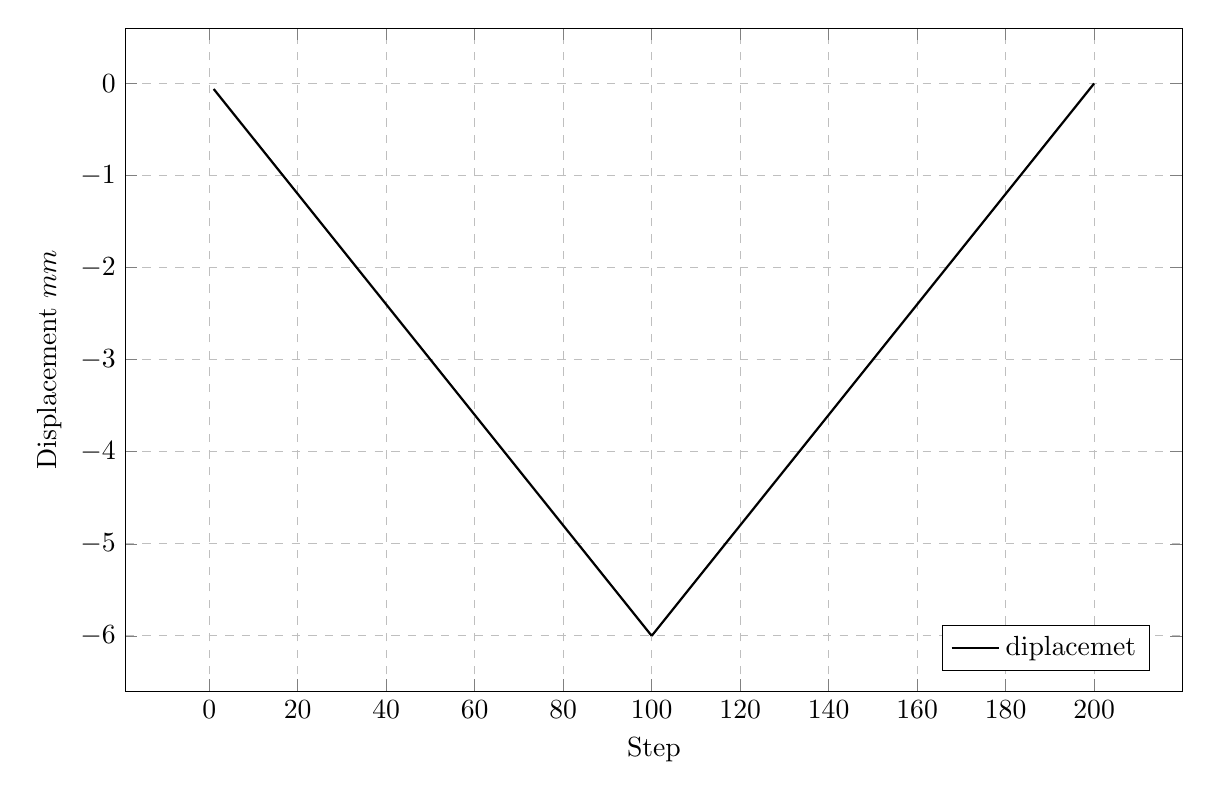
\begin{tikzpicture}
\pgfplotsset{major grid style={dashed},}
\begin{axis}[
						legend pos=south east,
						width=15cm,
						height=10cm,
						grid=major,
						ylabel=Displacement $mm$,
						xlabel=Step]
\addplot [thick, black, domain=1:100] {(-6/100)*x};
\addplot [thick, black, domain=100:200] {(6/100)*x-12};
\addlegendentry{diplacemet}
\end{axis}
\end{tikzpicture}}
    \caption{Load step die}
    \label{img:HW6-Displacement}
\end{figure}
It has opted for a high number of steps to avoid convergence problems during the solution phase, as in the first trials advised the program to increase the number of steps in the phase of application of the force as it was not able to find the solution after several iterations.
\section{Result and Conclusion}
%In the tuning options of the type \textsc{conta172} elements, you set the default method \emph{Augmented Lagrangian} as robust and present less sensitive to the magnitude of the contact stiffness.\\
The Von Mises equivalent stress at the end of the travel of the punch
and the maximum axial force applied to the punch, as show in figure \ref{img:HW6-Solu_101}.\\
\begin{figure}[!h]
\centering
\includegraphics[width=0.8\linewidth]{imgHW6/HW6-Solu_101}
\caption{Equivalent stress Von Mises}
\label{img:HW6-Solu_101}
\end{figure}\noindent
Max axial force applied to the punch is eqaul to $F = -58729,04097 \, N$.
\begin{figure}[!h]
\centering
    \resizebox{.8\linewidth}{!}{\begin{tikzpicture}
\pgfplotsset{cycle list={blue\\}, major grid style={dashed},}
\begin{axis}[
						legend pos=south east,
						width=15cm,
						height=10cm,
 						xmin=0, xmax=200,
        				ymin=-60000, ymax=1000,
        				grid=major,
        				ylabel=Force $N$,
        				xlabel=Step]
\addplot [thick, blue] table[smooth, mark=none, y=force, x=n]{HW6ForcePunch.txt};
\addlegendentry{Punch's force}
\end{axis}
\end{tikzpicture}}
    \caption{Force}
    \label{img:HW6-Force}
\end{figure}\\
%PARLARE HOOPSTRAIN
The punch stroke that maintains the maximum absolute, where is equal to $\sigma_{h} = 0,09445 \, MPa$, hence hoop stress close to the $5\,\%$ is equal $\sigma_{h5\%} = 0,0047 \, MPa$, hence the value of hoop strain is equal to $0,57169 \, mm$ as show in figure \ref{img:HW6-Hoopstrain}.
\begin{figure}[!h]
\centering
    \resizebox{.8\linewidth}{!}{\begin{tikzpicture}
\pgfplotsset{cycle list={orange\\pink\\purple\\red\\violet}, major grid style={dashed},}
\begin{axis}[
						width=15cm,
						height=10cm,
 						xmin=0, xmax=200,
        				grid= major,
        				xlabel=Step,
        				ylabel= Hoop strain $MPa$]
\addplot [thick, smooth, mark=none, Emerald] table [y={pHS}, x={n}]{HW6HoopStrain.txt};
\addplot [thick, smooth, mark=none, Emerald] table [y={nHS}, x={n}]{HW6HoopStrain.txt};
\draw [dash dot, red](axis cs:0,-0.0047) -- (axis cs:200,-0.0047) node [midway, above ] {
\textsc{\scriptsize \color{red}$5\,\%$}};
\draw [dash dot, red](axis cs:9.608941617,0) -- (axis cs:9.608941617,-0.0047);
\addlegendentry{Hoop strain}
\end{axis}
\end{tikzpicture}}
    \caption{Hoop strain below $5\, \%$}
    \label{img:HW6-Hoopstrain}
\end{figure}\\
When a metal forming tool is planned and designed to deform a work piece, the shape imparted by the tool will be a combination of elastic and plastic deformation, the release of the elastic deformation is the spring back often observed at the end of a metal forming process. The spring back has to be compensated to achieve an accurate result.\\The springback effect is visible in the follow graph \ref{img:HW6-Springback}.
\begin{figure}[!h]
\centering
    \resizebox{.8\linewidth}{!}{\begin{tikzpicture}
\pgfplotsset{cycle list={cyan\\magenta\\orange\\pink\\purple\\red\\teal\\violet\\yellow\\}, major grid style ={dashed, gray},}
\begin{axis}[
						legend cell align={left},
						legend pos=south east,
						width=15cm,
						height=10cm,
 						xmin=0, xmax=25,
        				ymin=-7, ymax=1,
						grid=major,
						xlabel=Radius $mm$,
						ylabel=Displacement $mm$]
\addplot [thick, smooth, mark=none] table[y=displacement, x=n]{HW6Set101.txt};
\addlegendentry{before remove punch}
\addplot +[stack plots=y, thick] table[smooth, mark=none, y=displacement, x=n ]{HW6Set103.txt};
\addlegendentry{after remove punch}
\addplot +[stack plots=y, stack dir=minus, thick ] table[smooth, mark=none, y=displacement, x=n]{HW6Set101.txt};
\addlegendentry{springback}
\end{axis}
\end{tikzpicture}}
    \caption{Springback effect}
    \label{img:HW6-Springback}
\end{figure}\\\noindent
Finally shows the plotted data showing the residual stress distribution on top and bottom surface of the blank after the punch removal, as in figures \ref{img:HW6-Solu_103}, \ref{img:HW6-TOP_Seqv} and \ref{img:HW6-BOT_Seqv}. 
\begin{figure}[!h]
\centering
\includegraphics[width=0.8\linewidth]{imgHW6/HW6-Solu_103}
\caption{Equivalent stress Von Mises}
\label{img:HW6-Solu_103}
\end{figure}
\begin{figure}[!h]
\centering
\includegraphics[width=0.8\linewidth]{imgHW6/HW6-TOP_SEQV}
\caption{Equivalent stress Von Mises top surface}
\label{img:HW6-TOP_Seqv}
\end{figure}
\begin{figure}[!h]
\centering
\includegraphics[width=0.8\linewidth]{imgHW6/HW6-BOT_SEQV}
\caption{Equivalent stress Von Mises bottom surface}
\label{img:HW6-BOT_Seqv}
\end{figure}
\clearpage
\section{Command list}
\begin{multicols}{2}
\scriptsize
\lstinputlisting[language=APDL, style=apdl-modified]{CommandList-HW6imgMOD.txt}
\normalsize
\end{multicols}
	\chapter{Homework 7}
\begin{minipage}{.70\textwidth}
\centering
\includegraphics[width=0.8\linewidth]{imgHW7/HW7}
\end{minipage}
\begin{minipage}{.70\textwidth}
\begin{tabular}{l}
        DATA:\\
        $\frac{D}{d} = 1.4 $\\
        $\frac{r}{d} = \frac{1}{20} $\\
        $R = \frac{(D-d)}{2}$\\
        Material: steel
\end{tabular}
\end{minipage}\\\\
Determine the stress concentration factor (defined as ratio between the maximum first principal stress in the model and the remote stress acting on the cross-secton with diameter d), in the presence and in the absence of the optimized relief groove analyzed in Homework 3, when the shaft is subject to uniform bending and torsional moment.
\section{Approach the problem}
In this issue we used the geometric model produced in homework 3, setting the \textsc{x} previously found at a value equal to $\textsc{x} = 1,5$ for the shaft with relief groove. Then going to replace the elements of the mesh with the type \textsc{Plane25}. The mesh is mapped with the same number of divisions seen in Homework 3, obtaining the result shown in figures \ref{img:HW7-Geometry}.\\
The material present the follow proprities:
\begin{itemize}
\item Modulus of elasticity: $210\, GPa$;
\item Poissons ratio $0.3$.
\end{itemize}
Assumptions adopted:
\begin{itemize}
\item Element type for both model \textsc{Plane25};
\item $x = 1.5$ optimal position;
\item Bending moment : $1*10^5 Nm$;
\item Torque moment: $1*10^6 Nm$;
\end{itemize}
\begin{figure}[htb]
\centering
\subfloat[][Gemotry - Shaft without relief groove]{\includegraphics[width=.7\textwidth]{/imgHW7/Part1/HW7-Geometry_PART1}} \\
\subfloat[][Gemotry - Shaft relief groove]{\includegraphics[width=.7\textwidth]{/imgHW7/Part2/HW7-Geometry_PART2}} 
\caption{Model of the shaft used in previous homework 3}
\label{img:HW7-Geometry}
\end{figure}
\begin{figure}[!h]
\centering
\subfloat[][Shaft without relief groove]{\includegraphics[width=.8\textwidth]{/imgHW3/Part1/HW3-Mesh_PART1}} \\
\subfloat[][Shaft relief groove]{\includegraphics[width=.8\textwidth]{/imgHW3//Part2/HW3-Mesh_PART2}}
\label{img:HW3-meshed}
\caption{Mapped mesh's model}
\end{figure}\pagebreak
\newpage
\section{Result}
An analysis is performed only by first applying a bending moment at the end of the two shafts and compared the values obtained in the presence or not of the relief groove.\\ It is repeated the same analysis this time, by applying a torque.
Finally, it analyzed the combination of the moments of both shafts.
The stress concentration factor subject to:
\subsection{Bending moment}
Impose a bending moment eqault to Mf $= 1 * 10^5 Nm$.\\
The stress concentration factor is defined as: $K_{t} = \frac{ \sigma_{1,max}}{S_{nom}}$, where $\sigma_{1,max}=$ maximum first principal stress in the model\\
\[S_{nom}= \frac{32Mf}{\pi d^3}=3,8340 \, MPa\]
\begin{table}[h]
\centering
\begin{tabular}{lcc}
\hline
& Maximim first principal  & stress concentraton factor\\
& stress in the model & of\\
& $\frac{N}{mm^2}$ &analysis\\
\hline
normal shaft & $\sigma_{1,max}= 8,55803 $ &$K_{t1}= 2,23$\\
shaft with relief groove & $\sigma_{1,max}=6,55013 $ &$K_{t1}=1,71$\\
\hline
\end{tabular}
\end{table}
Ratio of reduction $ = \frac{K_{t1}-K_{t2}}{K_{t1}}= 47,53 \%$
\begin{figure}[!h]
\centering
\includegraphics[width=.8\textwidth]{/imgHW7/Part1/HW7-MaxFirstStressBendingMoment_PART1}
\caption{Max First Stress Bending Moment - Shaft without relief groove}
\label{img:HW7-MFBM1}
\end{figure}
\begin{figure}
\centering
\includegraphics[width=.8\textwidth]{/imgHW7/Part2/HW7-MaxFirstStressBendingMoment_PART2}
\caption{Max First Stress Bending Moment - Shaft relief groove}
\label{img:HW7-MFBM2}
\end{figure}\\
%%%%%%%%%%%%%%%%%%%%%%%%%%%%%%%%%%%%%%%% 
\newpage
\subsection{Torque moment}
Impose a torque equal to Mt $= 1 * 10^6 Nm$.\\
The stress concentration factor is defined as: $K_{t}$ = $\frac{\sigma_{1,max}}{S_{nom}}$, where $\sigma_{1,max}=$ maximum first principal stress in the model\\
\[S_{nom}= \frac{16Mt}{\pi d^3}=19,1702 \, MPa\]
\begin{table}[h]
\centering
\begin{tabular}{lcc}
\hline
& Maximim first principal  & stress concentraton factor\\
& stress in the model & of\\
& $\frac{N}{mm^2}$ &analysis\\
\hline
normal shaft & $\sigma_{1,max}=61,2829 $ &$K_{t1}=3,19$\\
shaft with relief groove & $\sigma_{1,max}= 54,4842$ &$K_{t1}=2,84$\\
\hline
\end{tabular}
\end{table}
Ratio of reduction = $\frac{K_{t1}-K_{t2}}{K_{t1}}= 10,97\%$
\begin{figure}[!h]
\centering
\subfloat[][Shaft without relief groove]{\includegraphics[width=.8\textwidth]{/imgHW7/Part1/HW7-MaxFirstStressTorsionMoment_PART1}} \,
\subfloat[][Shaft relief groove]{\includegraphics[width=.8\textwidth]{/imgHW7/Part2/HW7-MaxFirstStressTorsionMoment_PART2}} 
\caption{Max First Stress Torsion Moment}
\label{img:HW7-MFTM}
\end{figure}
\pagebreak
%%%%%%%%%%%%%%%%%%%%%%%%%%%%%%%%%%
\newpage
\subsection{Combined moments}
For last analysis impose a combination of previuos bending moment and torque, Mf $= 1* 10^5 Nm$ and Mt $= 1 * 10^6 Nm$.
\begin{table}[h]
\centering
\begin{tabular}{lcc}
\hline
& Maximim first principal\\
& stress in the model\\
& $\frac{N}{mm^2}$\\
\hline
normal shaft & $\sigma_{1,max}= 66,7419$ \\
shaft with relief groove & $\sigma_{1,max}=58,3871 $\\
\hline
\end{tabular}
\end{table}
\begin{figure}[!h]
\centering
\subfloat[][Shaft without relief groove]{\includegraphics[width=.7\textwidth]{/imgHW7/Part1/HW7-MaxFirstStressCombMoment_PART1}} \,
\subfloat[][Shaft relief groove]{\includegraphics[width=.7\textwidth]{/imgHW7/Part2/HW7-MaxFirstStressCombMoment_PART2}} 
\caption{Max First Stress Combined Moment}
\label{img:HW7-MFCM}
\end{figure}\pagebreak
\section{Conclusion}
As we can see from results obtained, the stress concentration factor of the two cases, underlined that: in case of bending moment the presence of relief groove obtained a ratio of reduction of $47,53 \%$.
Otherwise in case of torque moment the ratio of reduction obtained $10,71 \%$.
Hence the presence of relief groove, decrease especially the bending stress concentration. In conclusion also in case of combined stress in presence of relief groove the stress state is more less than normal shaft.
\section{Command list}
\begin{multicols}{2}
\scriptsize
\lstinputlisting[language=APDL, style=apdl-modified]{CommandList-HW7.txt}
\lstinputlisting[language=APDL, style=apdl-modified]{CommandList-HW7Part2.txt}
\normalsize
\end{multicols}
	% Inserite qui gli altri capitoli:
	%%%%%%%%%%%%%%%%%%%%%%%%%%%%%%%%%%%%%%%%%%%%%%%%%%%%%%%%%%%%

\chapter{Conclusioni}
\label{ref:Conclusioni}

Spero che la guida possa servirvi ragazzuoli!\\\\

\noindent Ringrazio di cuore Giordano Cardillo e Matteo Merola per avermi aiutato (e sopportato) a capire come funziona questo maledetto \LaTeX ! :P

Ringraziate Giordano anche per aver creato dei loghi vettoriali decenti da utilizzare :D (li trovate nella cartella delle immagini).\\\\\noindent 

\noindent Vi voglio bene <3 (tranne a Rosangela u.u)\\\\

\begin{flushright}
\textit{Guida scritta da Lorenzo Valente} \footnote{http://facebook.com/lorenzo.valente}
\end{flushright}
\nocite{*}
	% === Bibliografia ====================================
	\newpage
	\bibliographystyle{IEEEtran}
	\bibliography{bibliografia-tesi.bib}

\end{document}
%========================================